% ****** Start of file aipsamp.tex ******
%
%   This file is part of the AIP files in the AIP distribution for REVTeX 4.
%   Version 4.1 of REVTeX, October 2009
%
%   Copyright (c) 2009 American Institute of Physics.
%
%   See the AIP README file for restrictions and more information.
%
% TeX'ing this file requires that you have AMS-LaTeX 2.0 installed
% as well as the rest of the prerequisites for REVTeX 4.1
% 
% It also requires running BibTeX. The commands are as follows:
%
%  1)  latex  aipsamp
%  2)  bibtex aipsamp
%  3)  latex  aipsamp
%  4)  latex  aipsamp
%
% Use this file as a source of example code for your aip document.
% Use the file aiptemplate.tex as a template for your document.
\documentclass[%
 aip,
% jmp,
% bmf,
% sd,
% rsi,
 amsmath,amssymb,
%preprint,%
 reprint, floatfix%
%author-year,%
%author-numerical,%
% Conference Proceedings
]{revtex4-1}

\usepackage{graphicx}% Include figure files
\usepackage{dcolumn}% Align table columns on decimal point
\usepackage{bm}% bold math
%\usepackage[mathlines]{lineno}% Enable numbering of text and display math
%\linenumbers\relax % Commence numbering lines

\usepackage[utf8]{inputenc}
\usepackage[T1]{fontenc}
\usepackage{mathptmx}
\usepackage{mathtools}
\usepackage{etoolbox}
\usepackage{booktabs}
\usepackage{multirow}
\usepackage{gensymb}
\usepackage{siunitx}
\usepackage[version=4]{mhchem}
\usepackage{bm}
\DeclareSIUnit\gauss{G}
\DeclareSIUnit{\angstrom}{\textup{\AA}}
\usepackage[hidelinks]{hyperref}
\hypersetup{
    colorlinks=true,
    linkcolor=blue,
    filecolor=magenta,      
    urlcolor=cyan,
    pdftitle={Overleaf Example},
    pdfpagemode=FullScreen,
    }

%% Apr 2021: AIP requests that the corresponding 
%% email to be moved after the affiliations
\makeatletter
\def\@email#1#2{%
 \endgroup
 \patchcmd{\titleblock@produce}
  {\frontmatter@RRAPformat}
  {\frontmatter@RRAPformat{\produce@RRAP{*#1\href{mailto:#2}{#2}}}\frontmatter@RRAPformat}
  {}{}
}%
\makeatother
\begin{document}

\preprint{AIP/123-QED}

\title[Frequency and temperature dependence of the dielectric constant]{Frequency and temperature dependence of the dielectric constant}
% Force line breaks with \\
\author{Maitrey Sharma}
 \affiliation{School of Physical Sciences, National Institute of Science Education and Research, HBNI, Jatni-752050, India.}%Lines break automatically or can be forced with \\
 \email{maitrey.sharma@niser.ac.in}

\date{\today}% It is always \today, today,
             %  but any date may be explicitly specified

\begin{abstract}
This experiment primarily deals with the study of the phenomena of Hall effect and magneto-resistance in semiconductors. First we explore the Drude model to lay down the foundation for the concepts and origin of Hall voltage and magneto-resistance and then using the well-known instrumentation like the four-probe, we establish various results. We determine the Hall coefficients of Bi, p-Ge and n-Ge and its relation to carrier density and carrier mobility, which are also determined for Bi. The unusual case of Bi is especially studied theoretically and experimentally. Then the magneto-resistance of Bi and n-Ge is determined and several plots are studied and results are drawn regarding them. 
\end{abstract}

\maketitle 


\begin{quotation}
\textit{Is it right to probe so deeply into Nature's secrets? The question must here be raised whether it will benefit mankind, or whether the knowledge will be harmful.}
\newline
\hspace*{0pt}\hfill Pierre Curie
\end{quotation}

\section{Introduction}
    In electromagnetism, a dielectric (or dielectric material or dielectric medium) is an electrical insulator that can be polarised by an applied electric field. When a dielectric material is placed in an electric field, electric charges do not flow through the material as they do in an electrical conductor, because they have no loosely bound, or free, electrons that may drift through the material, but instead they shift, only slightly, from their average equilibrium positions, causing dielectric polarisation. Because of dielectric polarisation, positive charges are displaced in the direction of the field and negative charges shift in the direction opposite to the field (for example, if the field is moving parallel to the positive x axis, the negative charges will shift in the negative x direction). This creates an internal electric field that reduces the overall field within the dielectric itself. If a dielectric is composed of weakly bonded molecules, those molecules not only become polarised, but also reorient so that their symmetry axes align to the field. The study of dielectric properties concerns storage and dissipation of electric and magnetic energy in materials.
    \begin{figure}
        \centering
        \includegraphics[scale = 0.25]{Figures/436px-Capacitor_schematic_with_dielectric.svg.png}
        \caption{A polarised dielectric material}
        \label{fig:dielectric}
    \end{figure}
    \par
    The absolute permittivity, often simply called permittivity ($\epsilon$) is a measure of the electric polarizability of a dielectric. A material with high permittivity polarizes more in response to an applied electric field than a material with low permittivity, thereby storing more energy in the material.
    \par
    In the simplest case, the electric displacement field $\mathbf{D}$ resulting from an applied electric field $\mathbf{E}$ is
    \begin{equation}
        \mathbf{D} = \epsilon \mathbf{E}
    \end{equation}
    More generally, the permittivity is a thermodynamic function of state. It can depend on the frequency, magnitude, and direction of the applied field. In this experiment we will study the variation of this permittivity or dielectric constant with frequency and temperature.
    \begin{figure}
        \centering
        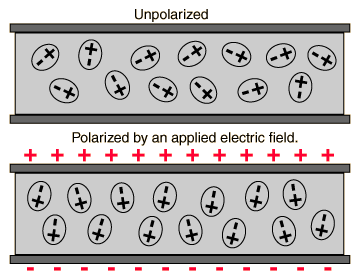
\includegraphics[scale = 0.5]{Figures/Diel.png}
        \caption{A dielectric medium showing orientation of charged particles creating polarization effects. Such a medium can have a lower ratio of electric flux to charge (more permittivity) than empty space}
        \label{fig:diel}
    \end{figure}

\section{Aim}
    The primary aim of this experiment is the study of frequency dependence of dielectric constant and ferroelectric to paraelectric phase transition of \ce{BaTiO3} by study of dielectric constant as a function of temperature and frequency.
\section{Apparatus}
    The apparatus used throughout the experiment is:
    \begin{enumerate}
        \item Probe arrangement: As shown in figure (\ref{fig:probe}), it has two spring loaded probes. These probes move in pipes and are insulated by Teflon bush, which ensure a good electrical insulation. The probe arrangement is mounted in suitable stand, which also hold the sample plate and RTD sensor. The RTD is mounted in the sample plates such that it is just below the sample, separated by a very thin sheet of mica. This ensures the correct measurement of sample temperature. This stand also serves as a lid of the oven. The leads are provided for the connection to RTD and capacitance meter,
        \begin{figure}
            \centering
            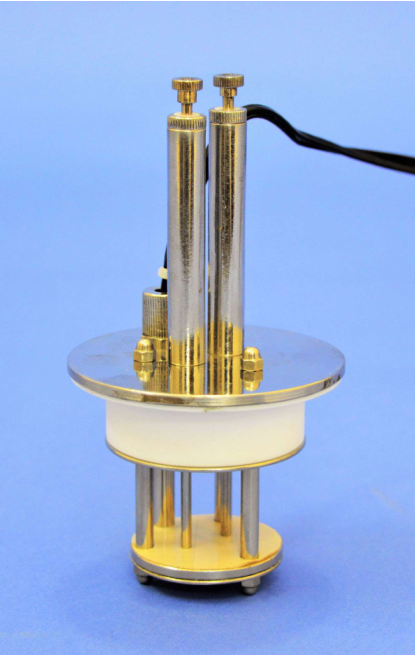
\includegraphics[scale = 0.4]{Figures/dielectric-arrange.png}
            \caption{Dielectric Constant Arrangement}
            \label{fig:probe}
        \end{figure}
        \item Barium titanate (\ce{BaTiO3}) plate with top and bottom conducting surface,
        \item Standard Multilayer Ceramic Capacitor,
        \item Disc Ceramic Capacitor,
        \item Main experimental setup unit
        \begin{figure}
            \centering
            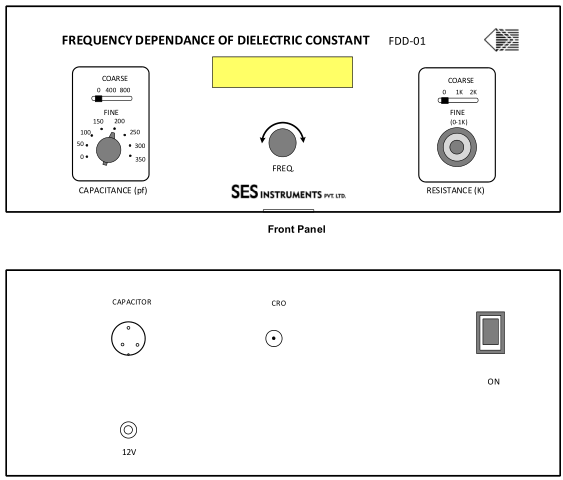
\includegraphics[scale = 0.6]{Figures/panel.png}
            \caption{Panel Diagram of the Unit}
            \label{fig:panel}
        \end{figure}
        \begin{figure}
            \centering
            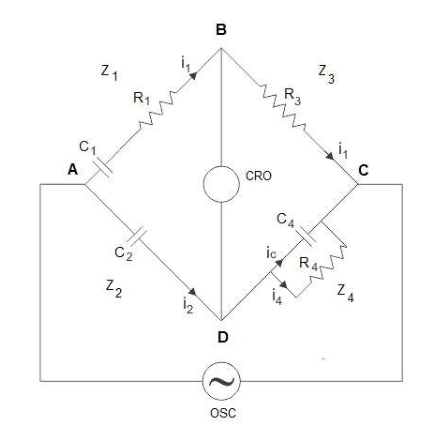
\includegraphics[scale = 0.8]{Figures/schering.png}
            \caption{Schering Bridge for Capacitance Measurement}
            \label{fig:schering}
        \end{figure}
        \item Oscilloscope
    \end{enumerate}
    The set-up consists of the main unit (figure (\ref{fig:panel})) for the measurement of capacitance at different frequencies from $\SI{1}{\kilo \hertz}$ to $\SI{50}{\kilo \hertz}$. This is done with the help of a Schering Bridge and a built-in oscillator. The basic bridge structure is shown in figure (\ref{fig:schering}).
    \par
    Here, $C_1$ is the unknown capacitance (\ce{BaTiO3}) whose value is to be determined with series electrical resistance $R_1$. $C_2$ is a standard silver mica capacitor of $\SI{1000}{\pico \farad}$. $C_4$ is a variable capacitor divided in two levels – Coarse and Fine. Coarse variation is divided in 3 steps and correspondingly Fine variation in further 8 steps. $R_3$ is a metal film resistance of $\SI{3.0}{\kilo \ohm}$. $R_4$ is a variable resistance, \textit{coarse} 0, 1k, 2k, 3k (selectable) in series with \textit{fine} 1k/10T potentiometer, connected in parallel with $C_4$.


\section{Theory}
    In the classical approach to the dielectric, the material is made up of atoms. Each atom consists of a cloud of negative charge (electrons) bound to and surrounding a positive point charge at its center. In the presence of an electric field, the charge cloud is distorted, as shown in figure (\ref{fig:dielectric-model}).
    \begin{figure}
        \centering
        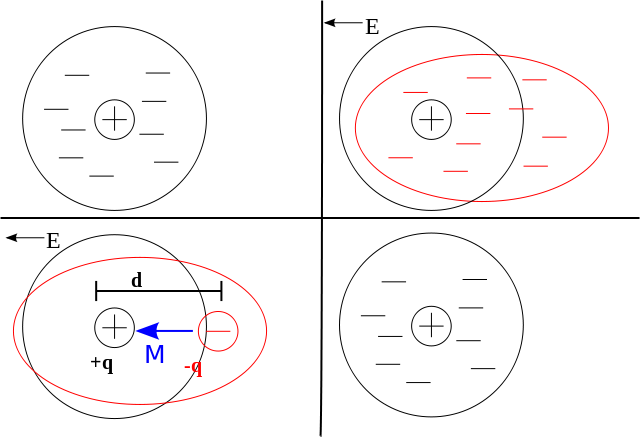
\includegraphics[scale = 0.35]{Figures/640px-Dielectric_model.svg.png}
        \caption{Electric field interaction with an atom under the classical dielectric model}
        \label{fig:dielectric-model}
    \end{figure}
    \par
    This can be reduced to a simple dipole using the superposition principle. A dipole is characterised by its dipole moment, a vector quantity shown in the figure as the blue arrow labeled M. It is the relationship between the electric field and the dipole moment that gives rise to the behaviour of the dielectric.
    \subsection{Complex Permittivity}
    As opposed to the response of a vacuum, the response of normal materials to external fields generally depends on the frequency of the field. This frequency dependence reflects the fact that a material's polarization does not change instantaneously when an electric field is applied. The response must always be causal (arising after the applied field), which can be represented by a phase difference. For this reason, permittivity is often treated as a complex function of the (angular) frequency $\omega$ of the applied field:
    \begin{equation}
        \epsilon \rightarrow \hat{\epsilon}(\omega)
    \end{equation}
    (since complex numbers allow specification of magnitude and phase). The definition of permittivity therefore becomes
    \begin{equation}
        D_0 e^{-i \omega t} = \hat{\epsilon}(\omega) E_0 e^{-i \omega t}
    \end{equation}
    where $D_0$ and $E_0$ are the amplitudes of the displacement and electric fields, respectively.
    \par
    At the plasma frequency and below, dielectrics behave as ideal metals, with electron gas behavior. The static permittivity is a good approximation for alternating fields of low frequencies, and as the frequency increases a measurable phase difference $\delta$ emerges between $\mathbf{D}$ and $\mathbf{E}$. The frequency at which the phase shift becomes noticeable depends on temperature and the details of the medium. For moderate field strength ($E_0$), $\mathbf{D}$ and $\mathbf{E}$ remain proportional, and
    \begin{equation}
        \hat{\epsilon} = \dfrac{D_0}{E_0} = \lvert \epsilon \rvert e^{-i \delta}
    \end{equation}
    Since the response of materials to alternating fields is characterized by a complex permittivity, it is natural to separate its real and imaginary parts, which is done by convention in the following way:
    \begin{equation}
        \hat{\epsilon}(\omega) = \epsilon'(\omega) - i \epsilon''(\omega) = \Bigg \lvert \dfrac{D_0}{E_0} \Bigg \rvert (\cos \delta - i \sin \delta)
    \end{equation}
    where $\epsilon'$ is the real part of the permittivity, $\epsilon''$ is the imaginary part of the permittivity and $\delta$ is the loss angle.
    \begin{figure}
        \centering
        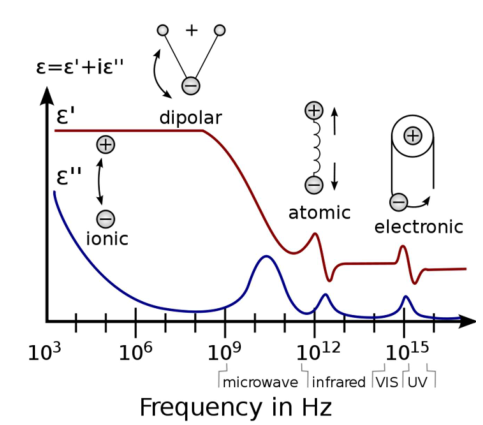
\includegraphics[scale = 0.8]{Figures/modelplot.png}
        \caption{Real and imaginary part of permittivity (dielectric constant) as function of frequency}
        \label{fig:model-plot}
    \end{figure}
    
    \subsection{Dielectric Polarization}
    Real part of permittivity depends on the polarizability. The total polarizability may usually be separated into three parts or four parts (when interfaces are involved): electronic, ionic (or atomic), dipolar (or orientation) and space charge. Each dielectric mechanism effect has a characteristic relaxation frequency. As the frequency becomes larger, the slower mechanisms drop off. This in turn leaves only the faster mechanisms to contribute to the dielectric storage or real part. The dielectric loss (imaginary part) will correspondingly peak at each critical frequency.
    \par
    Electronic polarization occurs in neutral atoms when an electric field displaces the nucleus with respect to the electrons that surround it. Atomic polarization occurs when neighboring positive and negative ions \textit{stretch} under an applied electric field. Both electronic and atomic polarization create induced moments depending on the polarizability of the atoms or molecules. A permanent dipole moment is caused by unbalanced sharing of electrons by atoms of a molecule. In an absence of an external electric field, these moments are oriented in a random order such that no net polarization is present. Under an external electric field, the dipoles rotate to align with the electric field causing orientation polarization to occur. The ionic polarization is composed of ionic conductivity and interfacial or space charge polarization. At low frequencies ionic conduction is the most prevalent mechanism. Ionic conduction only introduces losses into a system. Space charge polarization occurs when more than one material component is present or when segregation occurs in a material containing incompatible chemical sequences and when translating charge carriers become trapped at the interfaces of these heterogeneous systems. The electric field distortion caused by the accumulation of these charges increases the overall capacitance of a material which appears as an increase in real part of dielectric constant.
    \par
    The dielectric permittivity at optical frequencies arises almost entirely from the electronic polarizability.
    \subsection{Dielectric Heating}
    Both real and imaginary part are important for applications. For example, in the microwave heating, the dielectric constant ($\epsilon'$) represents a measure of the ability of a material to be polarized by an external electric field (as that of microwaves) storing energy within it. On the other hand, the dielectric loss factor ($\epsilon''$) represents the ability of the material to dissipate the absorbed electromagnetic energy, converting it into heat. The higher the dissipation capacity for a sample the lesser will be the penetration of microwaves into the same sample. Thus, the ratio ($\epsilon''/\epsilon'$) suggests the capability of each material to convert electromagnetic energy (microwaves) into heat at specific temperatures and frequencies.
    \par
    The loss factor is defined as
    \begin{equation}
        \tan \delta = \dfrac{\epsilon'_r}{\epsilon''_r}
    \end{equation}
    
    \subsection{Barium titanate}
    Barium titanate has a very large room temperature dielectric constant. It has perovskite structure. Perovskite is a family name of a group of materials and the mineral name of calcium titanate (\ce{CaTiO3}) having a structure of the type ABO\textsubscript{3}. Many piezoelectric (including ferroelectric) ceramics such as Barium titanate (\ce{BaTiO3}), Lead titanate (\ce{PbTiO3}), Potassium niobate (\ce{KNbO3}) etc. have a cubic perovskite type structure (in the paraelectric state) with chemical formula $ABO_3$ (figures (\ref{fig:pero1}), (\ref{fig:pero2})).
    \begin{figure}
        \centering
        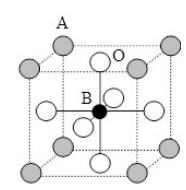
\includegraphics{Figures/abo3.png}
        \caption{Perovskite ABO\textsubscript{3} structure with the A and B cations on the corner and body centre positions, respectively. Three oxygen anions per unit cell occupy the faces and form octahedra surrounding the B-site.}
        \label{fig:pero1}
    \end{figure}
    \begin{figure}
        \centering
        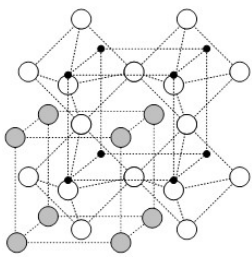
\includegraphics{Figures/batio3.png}
        \caption{Perovskite structure (Ba: Grey; Ti: Black; O: White)}
        \label{fig:pero2}
    \end{figure}
    \begin{figure}
        \centering
        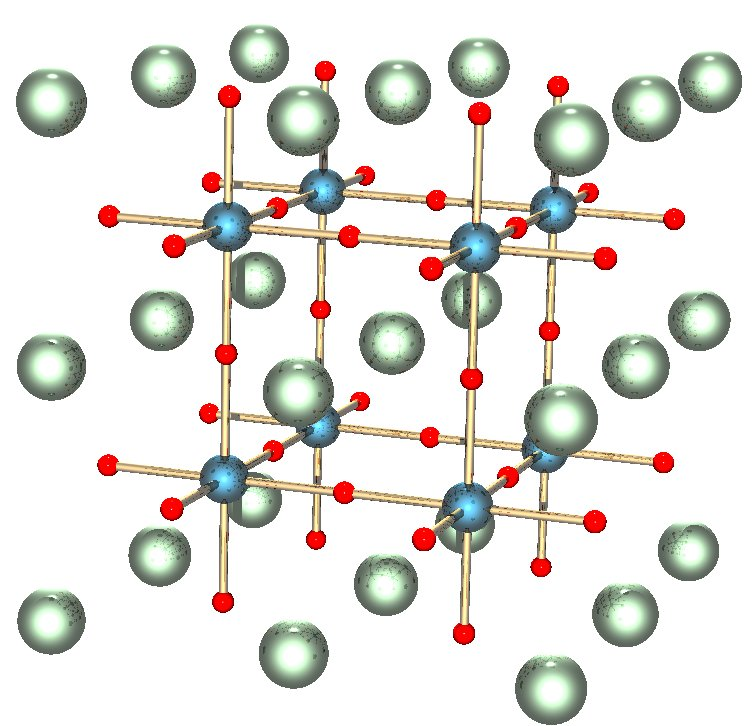
\includegraphics[scale = 0.3]{Figures/Perovskite.jpg}
        \caption{Structure of cubic \ce{BaTiO3}. The red spheres are oxide centres, blue are Ti\textsuperscript{4+} cations, and the green spheres are Ba\textsuperscript{2+}}
        \label{fig:my_label}
    \end{figure}
    \par
    As conventionally drawn, A-site cations occupy the corners of a cube, while B-site cations sit at the body centre. Three oxygen atoms per unit cell rest on the faces. The lattice constant of these perovskite is always close to the $\SI{4}{\angstrom}$ due to rigidity of the oxygen octahedral network and the well-defined oxygen ionic radius of $\SI{1.35}{\angstrom}$.
    \par
    A practical advantage of the perovskites structure is that many different cations can be substituted on both the A and B sites without drastically changing the overall structure. Complete solid solutions are easily formed between many cations, often across the entire range of composition. Even though two cations are compatible in solution, their behaviour can be radically different when apart from each other. Thus, it is possible to manipulate a material's properties such as Curie Temperature or dielectric constant with only a small substitution of a given caution.
    \par
    Barium Titanate (\ce{BaTiO3}) has a ferroelectric tetragonal phase below its curie point of about $\SI{120}{\celsius}$ and paraelectric cubic phase above Curie point. The temperature of the Curie point appreciably depends on the impurities present in the sample and the synthesis process.
    \par
    In the paraelectric cubic phase the centre of positive charges (Ba\textsuperscript{2+}, Ti\textsuperscript{4+}) coincide with the centre of negative charges (O\textsuperscript{2-} ion) and on cooling below $T_C$, a tetragonal phase develops where the centre of Ba\textsuperscript{2+} and Ti\textsuperscript{4+} ions are displaced relative to the O\textsuperscript{2-} ions, leading to the formation of electric dipoles.
    \par
    As the barium titanate ceramics have a very large room temperature dielectric constant, they are mainly used in multilayer capacitor applications. The grain size control of these polycrystalline sample used in the experiment is very important for these applications.
    
    \subsection{Ferroelectricity, Paraelectricity and Curie Temperature}
    Ferroelectricity is a characteristic of certain materials that have a spontaneous electric polarization that can be reversed by the application of an external electric field. All ferroelectrics are pyroelectric\footnote{property of certain crystals which are naturally electrically polarized and as a result contain large electric fields; can be described as the ability of certain materials to generate a temporary voltage when they are heated or cooled.}, with the additional property that their natural electrical polarization is reversible. The term is used in analogy to ferromagnetism, in which a material exhibits a permanent magnetic moment. Ferromagnetism was already known when ferroelectricity was discovered in 1920 in Rochelle salt by Valasek.
    \par
    When most materials are electrically polarized, the polarization induced, $P$, is almost exactly proportional to the applied external electric field $E$; so the polarization is a linear function. This is called linear dielectric polarization (figure (\ref{fig:linearpolar})). Some materials, known as paraelectric materials, show a more enhanced nonlinear polarization (figure (\ref{fig:para})). The electric permittivity, corresponding to the slope of the polarization curve, is not constant as in linear dielectrics but is a function of the external electric field.
    \begin{figure}
        \centering
        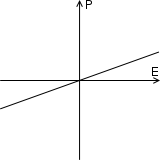
\includegraphics{Figures/lindielectric.png}
        \caption{Linear dielectric polarization}
        \label{fig:linearpolar}
    \end{figure}
    \begin{figure}
        \centering
        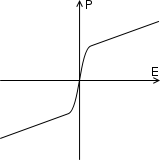
\includegraphics{Figures/160px-Paraelectric_polarisation.svg.png}
        \caption{Paraelectric polarization}
        \label{fig:para}
    \end{figure}
    \par
    In addition to being nonlinear, ferroelectric materials demonstrate a spontaneous nonzero polarization (figure (\ref{fig:ferro})) even when the applied field E is zero. The distinguishing feature of ferroelectrics is that the spontaneous polarization can be reversed by a suitably strong applied electric field in the opposite direction; the polarization is therefore dependent not only on the current electric field but also on its history, yielding a hysteresis loop. They are called ferroelectrics by analogy to ferromagnetic materials, which have spontaneous magnetization and exhibit similar hysteresis loops.
    \begin{figure}
        \centering
        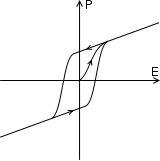
\includegraphics{Figures/160px-Ferroelectric_polarisation.svg.png}
        \caption{Ferroelectric polarization}
        \label{fig:ferro}
    \end{figure}
    \par
    Typically, materials demonstrate ferroelectricity only below a certain phase transition temperature, called the Curie temperature ($T_C$) and are paraelectric above this temperature: the spontaneous polarization vanishes, and the ferroelectric crystal transforms into the paraelectric state. Many ferroelectrics lose their pyroelectric properties above $T_C$ completely, because their paraelectric phase has a centrosymmetric crystal structure.
    \par
    The Curie temperature is named after Pierre Curie, who showed that magnetism was lost at a critical temperature.
    \subsection{The Schering Bridge}
    This circuit component is a important part of the experiment. Figure (\ref{fig:schering2}) shows the configuration of the Schering Bridge where $C_1$ is the unknown capacitance with series electrical resistance $R_1$, $C_2$ is a standard capacitor, $C_4$ is a variable capacitor, $R_3$ is a pure resistor (i.e. non inductive in nature), and, $R_4$ is a variable non inductive resistor connected in parallel with variable capacitor $C_4$.
    \begin{figure}
        \centering
        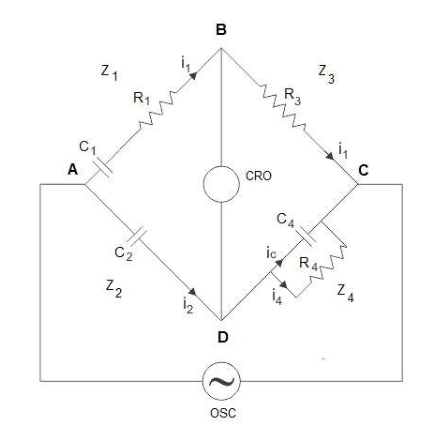
\includegraphics[scale = 0.95]{Figures/schering.png}
        \caption{The Schering Bridge}
        \label{fig:schering2}
    \end{figure}
    Now the supply is given to the bridge between the points A and C, and the detector (Oscilloscope) is connected between B and D. In the balance condition the Oscilloscope shows zero signal, i.e., there is no potential difference between points B and D. This implies the balance equation as,
    \begin{equation}
        Z_1/Z_3 = Z_2/Z_4
    \end{equation}
    From here, upon solving the equations in terms of impedance and resistances and comparing the real and imaginary parts we get
    \begin{equation}
        R_1 = \dfrac{R_3 C_4}{C_2}
    \end{equation}
    and
    \begin{equation}
        C_1 = \dfrac{R_4 C_2}{R_3}
    \end{equation}
    The unknown capacitor and its equivalent series resistance may therefore be computed from the above equation.
    \par
    The equivalent series resistance or ESR of a capacitor act like any other resistor giving rise to voltage drops and energy dissipated as heat. Although the ESR figure of a capacitor is mentioned more often, dissipation factor and loss tangent are also widely used and closely associated with the capacitor ESR. When a sinusoidal alternating voltage is applied to an ideal capacitor, the current leads by $\pi/2$ in phase. In the case of a practical capacitor, however, advance in phase is ($\pi/2 - \delta$), which is smaller than $\pi/2$. $\delta$ is referred to as the \textit{loss angle}.
\section{Observations}
    Following preliminary observations for \ce{BaTiO3} were made: diameter, $d = \SI{10.65}{\milli \metre}$ and thickness, $t = \SI{2.24}{\milli \metre}$. This implies area of the sample is $A = \SI{89.02}{\per \milli \metre \squared}$. As permittivity of space is given by $\epsilon_0 = \SI{8.85e-3}{\pico \farad \per \milli \metre}$, we can write $C_0 = \epsilon_0 A/t = \SI{0.35}{\pico \farad}$. Now, $\epsilon = C_1/C_0$. $R_4$ is the dial reading of resistance and from discussion on the Schering bridge, we have $C_1 = C_2 (R_4/R_3)$ with $C_2 = \SI{1000}{\pico \farad}$ and $R_3 = \SI{3}{\kilo \ohm}$.
    \par
    For the multi-layer ceramic capacitor and the disc ceramic capacitor, in the absence of dimensional information of commercially available capacitors, the value of $C_0$ cannot be computed. Hence, we tabulate value of capacitance, which is proportional to the dielectric constant, as a function of frequency in table (\ref{tab:mlcc}) and (\ref{tab:disc}). The respective plots between variation of capacitance with frequency are shown in figures (\ref{fig:mlcc}) and (\ref{fig:disc}). 
    \par
    The data for variation of capacitance parameters ($C_1$ and $R_1$) and dielectric constant as a function of frequency for \ce{BaTiO3} is tabulated in (\ref{tab:batio3}). Figure (\ref{fig:batio3}) shows the variation of dielectric constant of \ce{BaTiO3} with frequency over a frequency range of 0 to 50 kHz. This follows the same general variation as shown in figure (\ref{fig:model-plot}) over this frequency range.
    \par
    Figure (\ref{fig:diss}) shows the variation of the dissipation factor of barium titanate sample with frequency.
    \par
    The temperature dependence of dielectric constant at various frequencies is tabulated in table (\ref{tab:temp-batio3}) and the corresponding plot is given in figure (\ref{fig:curie}). 
    \par
    The diffuseness parameter, $\delta$, is defined as the slope of the plot between $\ln \Big( \dfrac{1}{\epsilon} - \dfrac{1}{\epsilon_{max}} \Big)$ versus $\ln (T- T_C)$, where $\epsilon$ is the dielectric constant at a temperature $T$, $\epsilon_{max}$ is the maximum value of the dielectric constant at the curie temperature, $T_C$, which corresponds to the peaks in the plot of variation of dielectric constant with temperature (figure (\ref{fig:curie})). The above is valid in the paraelectric phase, i.e., only beyond the Curie temperature. Therefore, the values of dielectric constant and other parameters after phase transition at the Curie temperature $T_C$ are tabulated in table (\ref{tab:delta}) and the corresponding plots between $\ln \Big( \dfrac{1}{\epsilon} - \dfrac{1}{\epsilon_{max}} \Big)$ and $\ln (T- T_C)$ for different frequencies are plotted in figure (\ref{fig:delta}). The slopes in figure (\ref{fig:delta}) represent the diffuseness parameter $\delta$.
    
    \begin{table}[]
    \caption{Variation of unknown capacitance as a function of frequency for multi-layer ceramic capacitor (MLCC)}
    \label{tab:mlcc}
    \setlength{\tabcolsep}{23pt}
    \begin{tabular}{@{}cccc@{}}
    \toprule
    \begin{tabular}[c]{@{}c@{}}\textbf{Frequency} $f$\\ ($\si{\kilo \hertz}$)\end{tabular} & \begin{tabular}[c]{@{}c@{}}$C_4$\\ ($\si{\pico \farad}$)\end{tabular} & \begin{tabular}[c]{@{}c@{}}$R_4$\\ ($\si{\ohm}$)\end{tabular} & \begin{tabular}[c]{@{}c@{}}$C_1$\\ ($\si{\pico \farad}$)\end{tabular} \\ \midrule
    1 & 500 & 1780 & 593.33 \\
    3 & 600 & 1764 & 588.00 \\
    5 & 600 & 1758 & 586.00 \\
    7 & 600 & 1762 & 587.33 \\
    10 & 600 & 1738 & 579.33 \\
    15 & 600 & 1742 & 580.67 \\
    20 & 600 & 1710 & 570.00 \\
    25 & 600 & 1714 & 571.33 \\
    30 & 600 & 1664 & 554.67 \\
    35 & 600 & 1658 & 552.67 \\
    40 & 600 & 1626 & 542.00 \\
    50 & 600 & 1580 & 526.67 \\ \bottomrule
    \end{tabular}
    \end{table}
    \begin{figure}
        \centering
        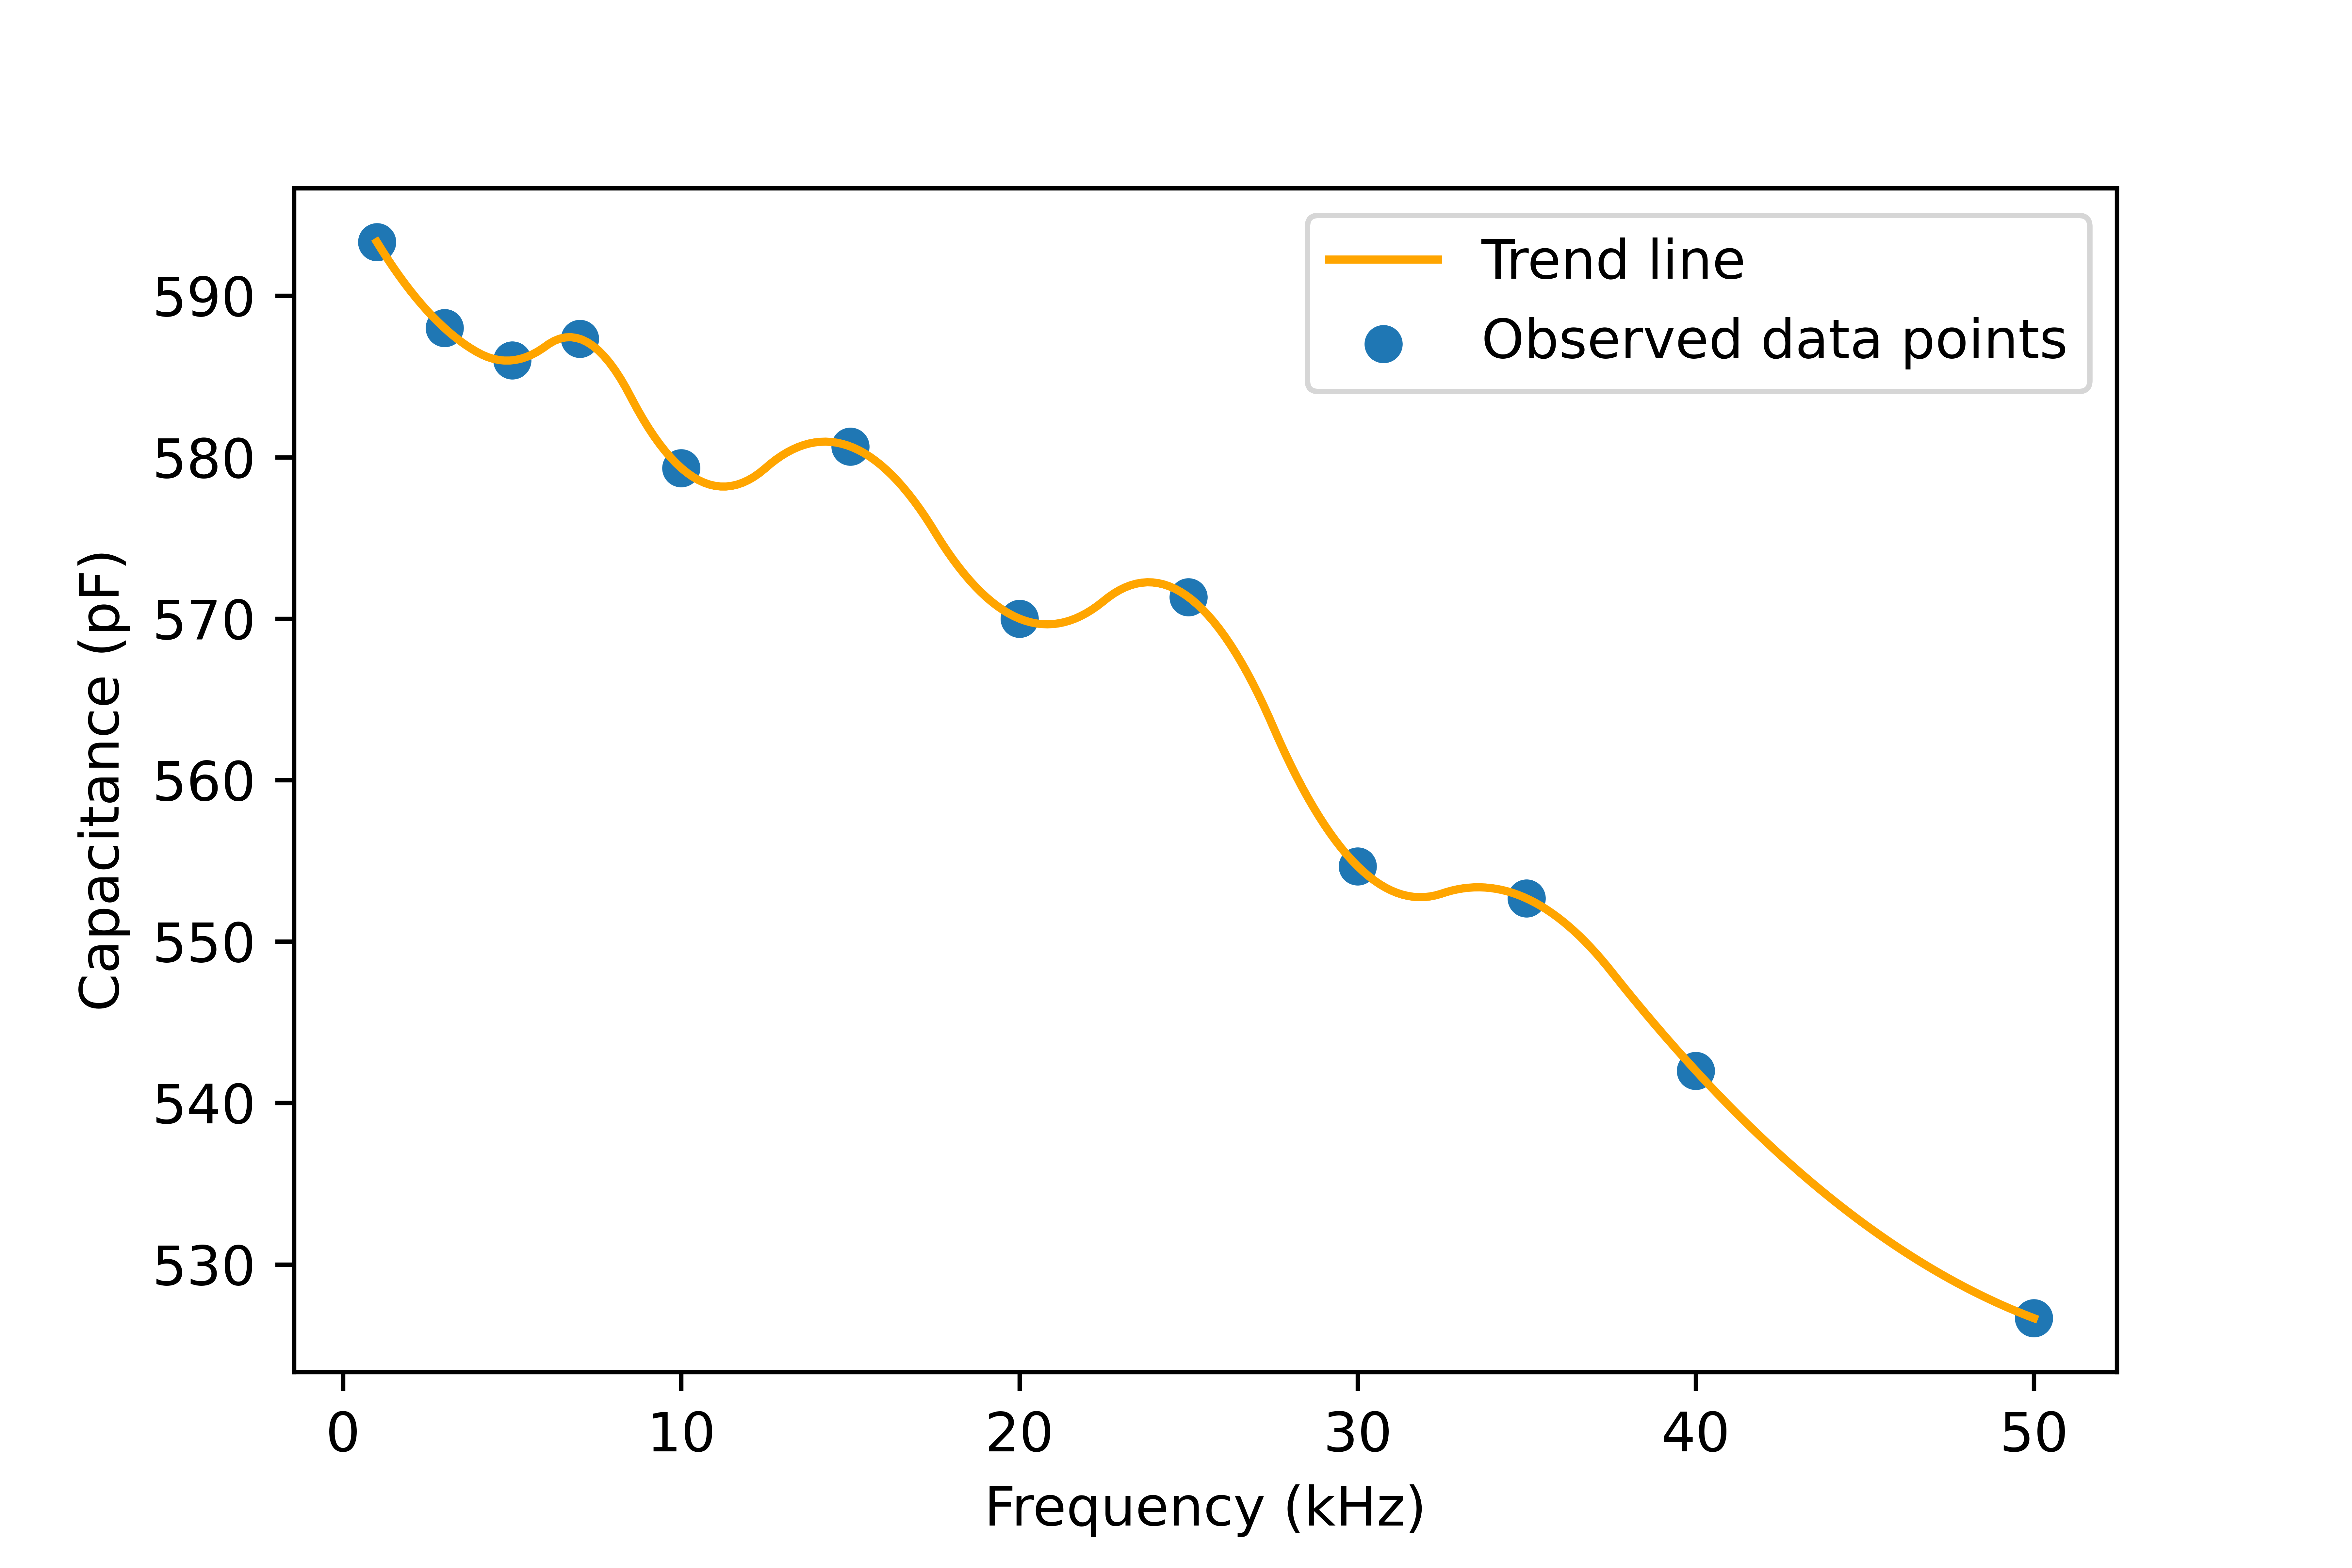
\includegraphics[scale = 0.56]{Figures/plot-mlcc.png}
        \caption{Variation of unknown capacitance as a function of frequency for multi-layer ceramic capacitor (MLCC)}
        \label{fig:mlcc}
    \end{figure}
    \begin{table}[]
    \caption{Variation of unknown capacitance as a function of frequency for disc ceramic capacitor}
    \label{tab:disc}
    \setlength{\tabcolsep}{23pt}
    \begin{tabular}{@{}cccc@{}}
    \toprule
    \begin{tabular}[c]{@{}c@{}}\textbf{Frequency} $f$\\ ($\si{\kilo \hertz}$)\end{tabular} & \begin{tabular}[c]{@{}c@{}}$C_4$\\ ($\si{\pico \farad}$)\end{tabular} & \begin{tabular}[c]{@{}c@{}}$R_4$\\ ($\si{\ohm}$)\end{tabular} & \begin{tabular}[c]{@{}c@{}}$C_1$\\ ($\si{\pico \farad}$)\end{tabular} \\ \midrule
    1 & 500 & 1918 & 639.33 \\
    2 & 500 & 1890 & 630.00 \\
    5 & 500 & 1882 & 627.33 \\
    7 & 500 & 1876 & 625.33 \\
    10 & 500 & 1872 & 624.00 \\
    15 & 500 & 1882 & 627.33 \\
    20 & 500 & 1870 & 623.33 \\
    25 & 500 & 1876 & 625.33 \\
    30 & 500 & 1828 & 609.33 \\
    35 & 500 & 1798 & 599.33 \\
    40 & 500 & 1794 & 598.00 \\
    50 & 500 & 1778 & 592.67 \\ \bottomrule
    \end{tabular}
    \end{table}
    \begin{figure}
        \centering
        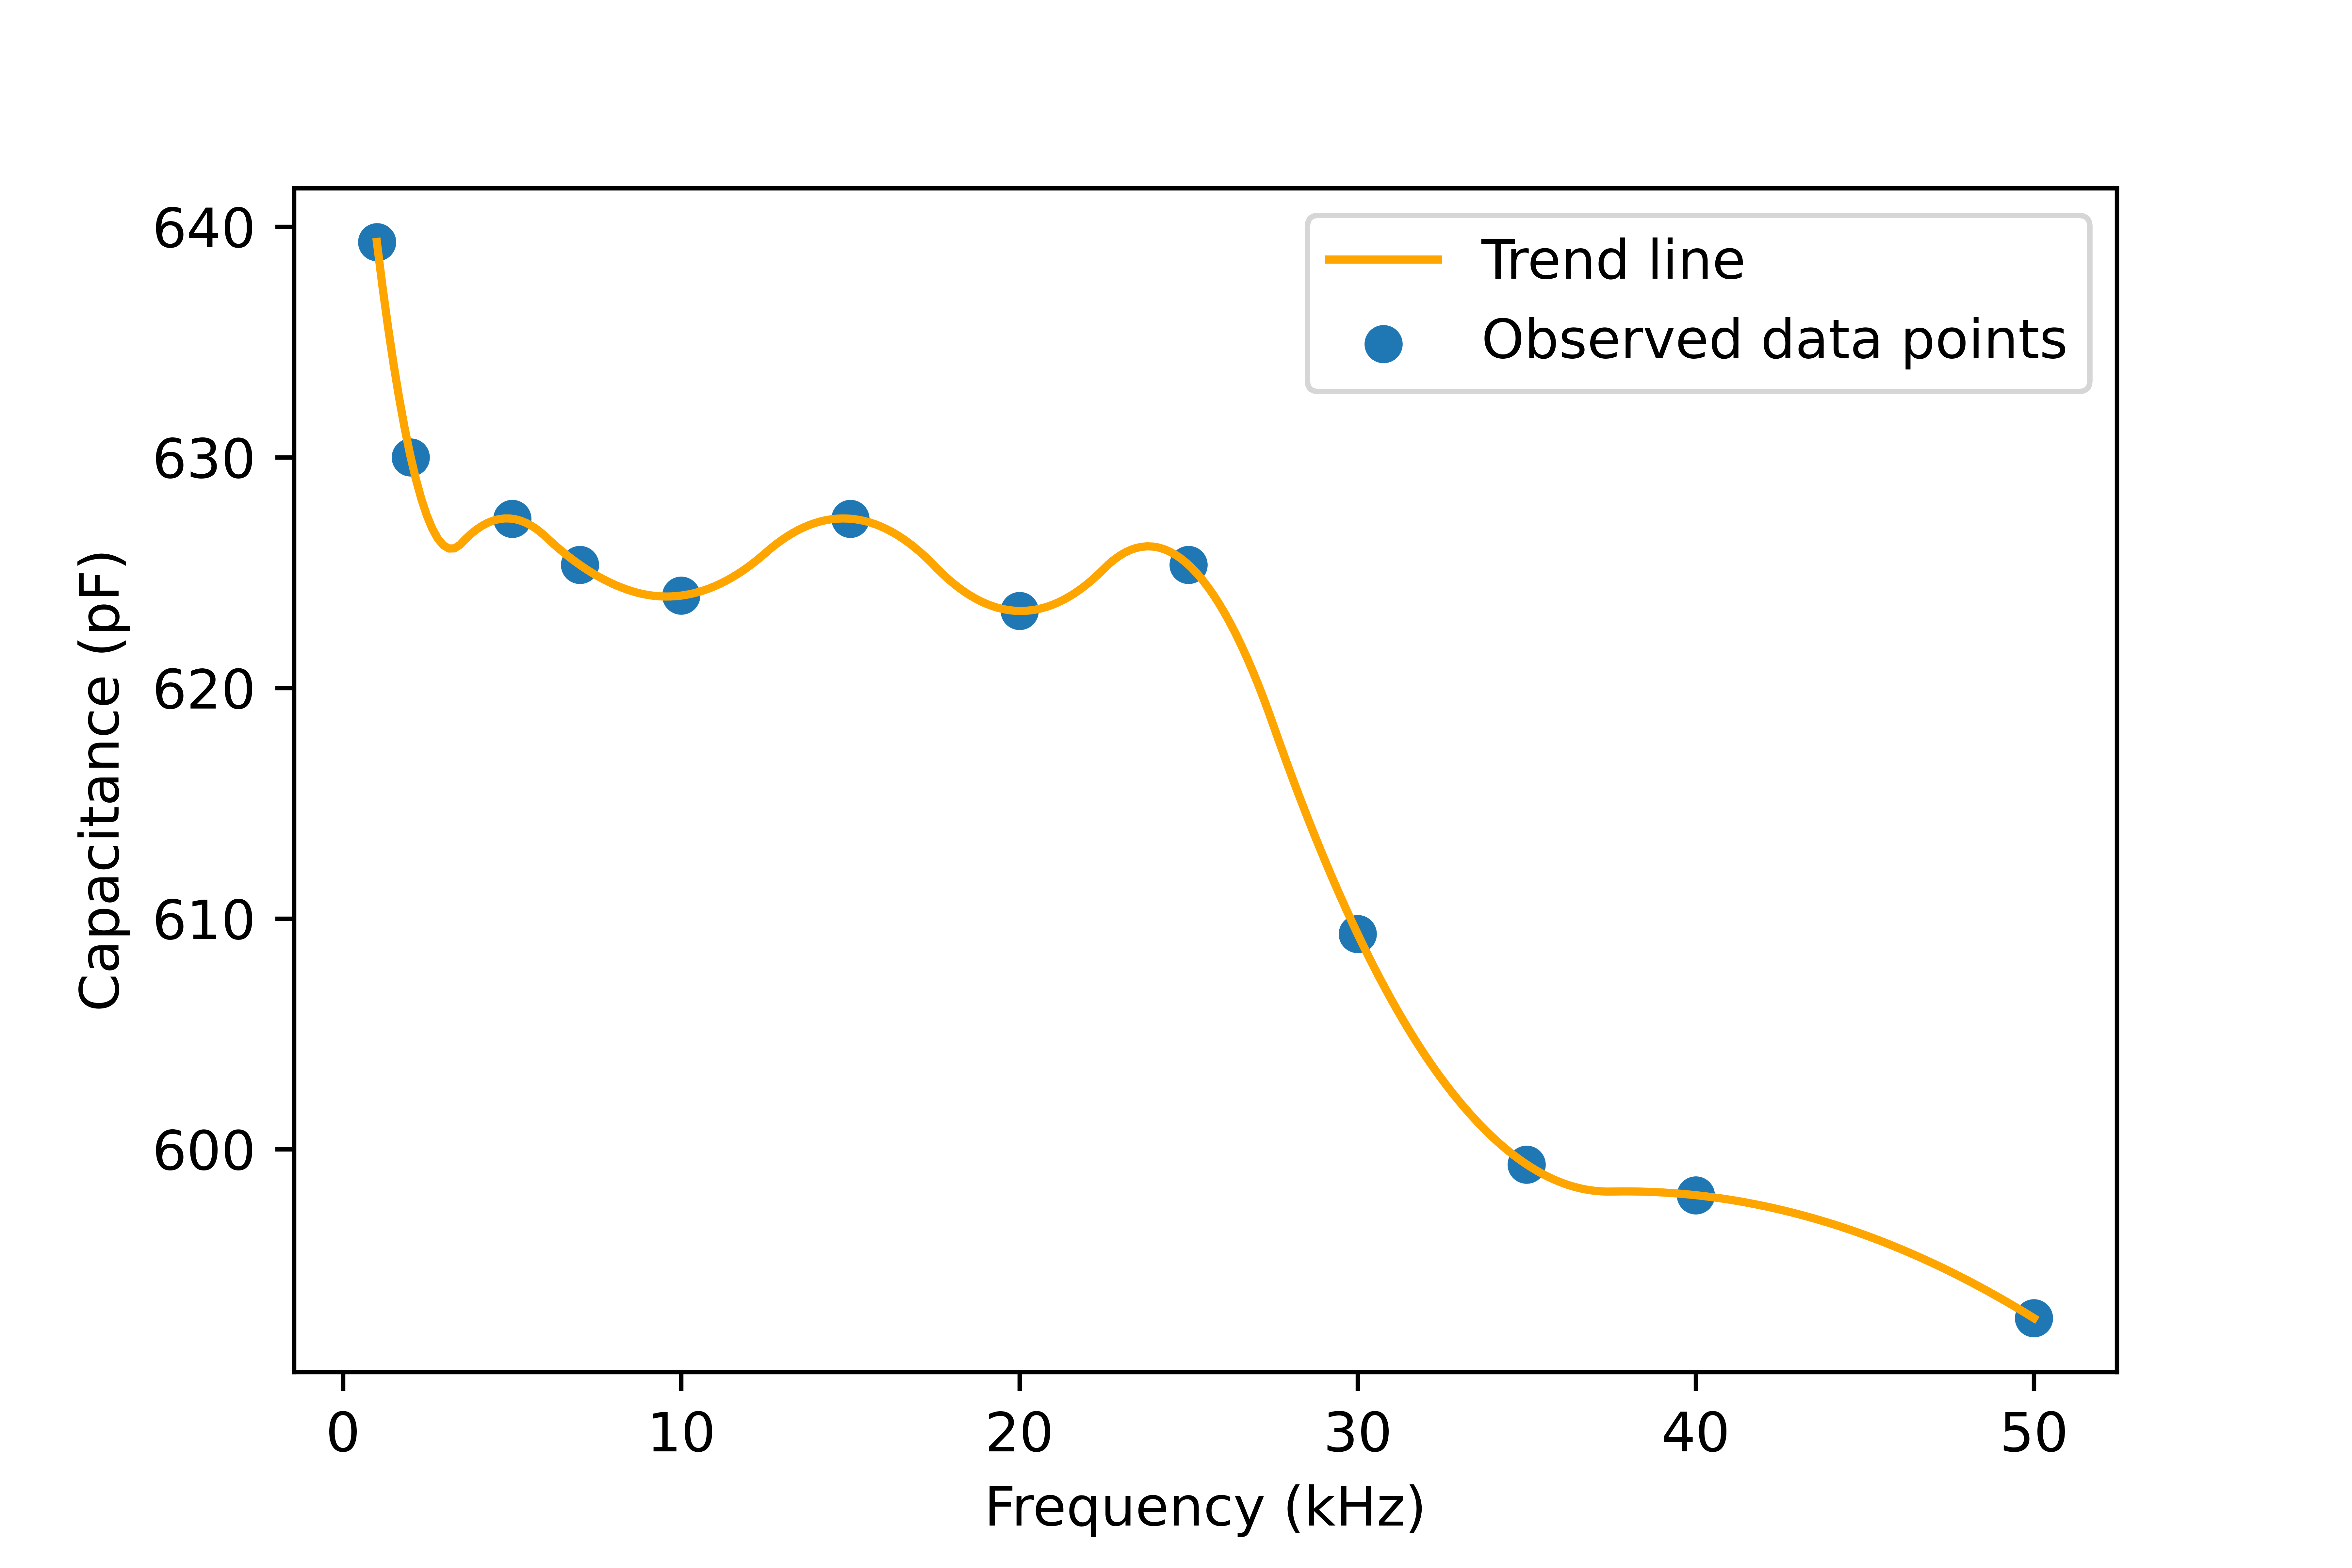
\includegraphics[scale = 0.56]{Figures/plot-ceramic.png}
        \caption{Variation of unknown capacitance as a function of frequency for disc ceramic capacitor}
        \label{fig:disc}
    \end{figure}
    \begin{table*}[]
    \caption{Variation of capacitance parameters ($C_1$ and $R_1$) and dielectric constant as a function of frequency}
    \label{tab:batio3}
    \setlength{\tabcolsep}{20pt}
    \begin{tabular}{@{}ccccccc@{}}
    \toprule
    \begin{tabular}[c]{@{}c@{}}\textbf{Frequency} $f$\\ ($\si{\kilo \hertz}$)\end{tabular} & \begin{tabular}[c]{@{}c@{}}$C_4$\\ ($\si{\pico \farad}$)\end{tabular} & \begin{tabular}[c]{@{}c@{}}$R_4$\\ ($\si{\ohm}$)\end{tabular} & \begin{tabular}[c]{@{}c@{}}$C_1$\\ ($\si{\pico \farad}$)\end{tabular} & \begin{tabular}[c]{@{}c@{}}$R_1$\\ ($\si{\ohm}$)\end{tabular} & \begin{tabular}[c]{@{}c@{}}\textbf{Dielectric constant}\\ ($\epsilon = C_0/C_1$)\end{tabular} & \begin{tabular}[c]{@{}c@{}}\textbf{Dissipation factor}\\ ($2 \pi f C R$)\end{tabular} \\ \midrule
    1 & 500 & 1940 & 646.7 & 1500 & 1838.30 & 0.006 \\
    3 & 500 & 1890 & 630.0 & 1500 & 1790.92 & 0.018 \\
    5 & 500 & 1866 & 622.0 & 1500 & 1768.18 & 0.029 \\
    7 & 500 & 1860 & 620.0 & 1500 & 1762.49 & 0.041 \\
    10 & 500 & 1848 & 616.0 & 1500 & 1751.12 & 0.058 \\
    15 & 500 & 1828 & 609.3 & 1500 & 1732.17 & 0.086 \\
    20 & 500 & 1816 & 605.3 & 1500 & 1720.80 & 0.114 \\
    25 & 500 & 1798 & 599.3 & 1500 & 1703.74 & 0.141 \\
    30 & 500 & 1792 & 597.3 & 1500 & 1698.06 & 0.169 \\
    35 & 500 & 1768 & 589.3 & 1500 & 1675.32 & 0.194 \\
    40 & 500 & 1746 & 582.0 & 1500 & 1654.47 & 0.219 \\
    50 & 500 & 1730 & 576.7 & 1500 & 1639.31 & 0.272 \\ \bottomrule
    \end{tabular}
    \end{table*}
    \begin{figure}
        \centering
        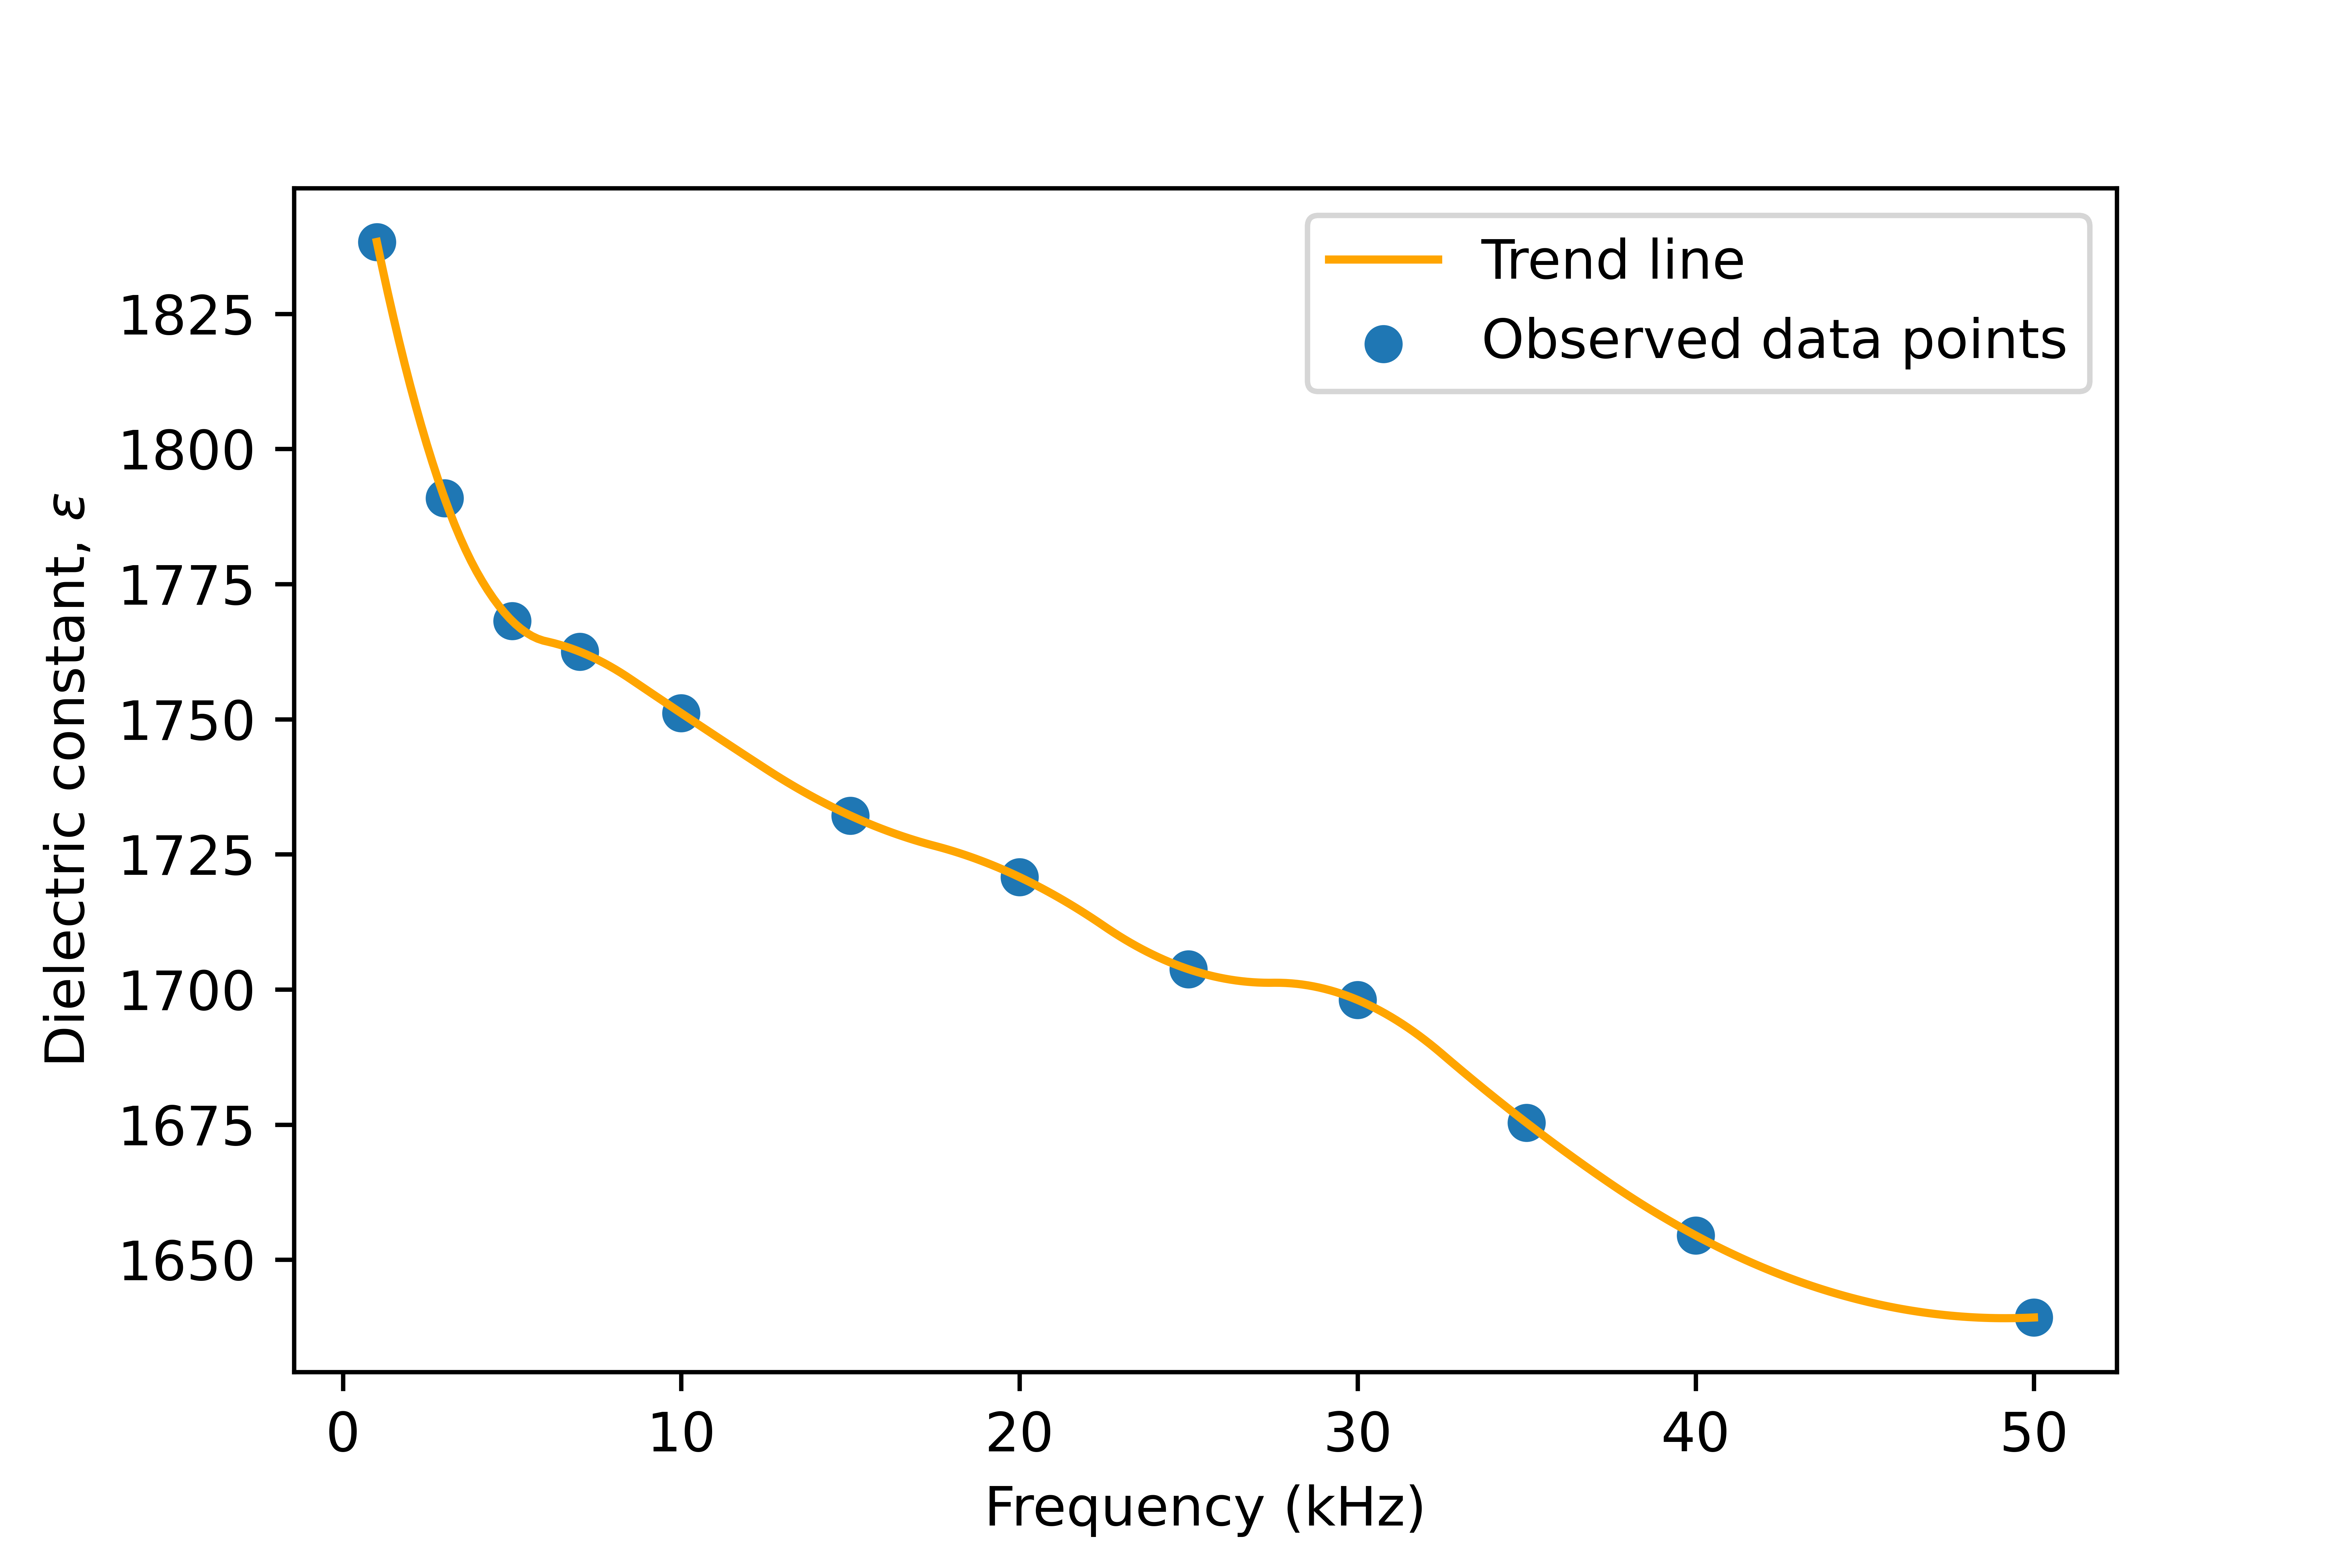
\includegraphics[scale = 0.56]{Figures/plot-batio3.png}
        \caption{Variation of dielectric constant as a function of frequency for \ce{BaTiO3}}
        \label{fig:batio3}
    \end{figure}
    \begin{figure}
        \centering
        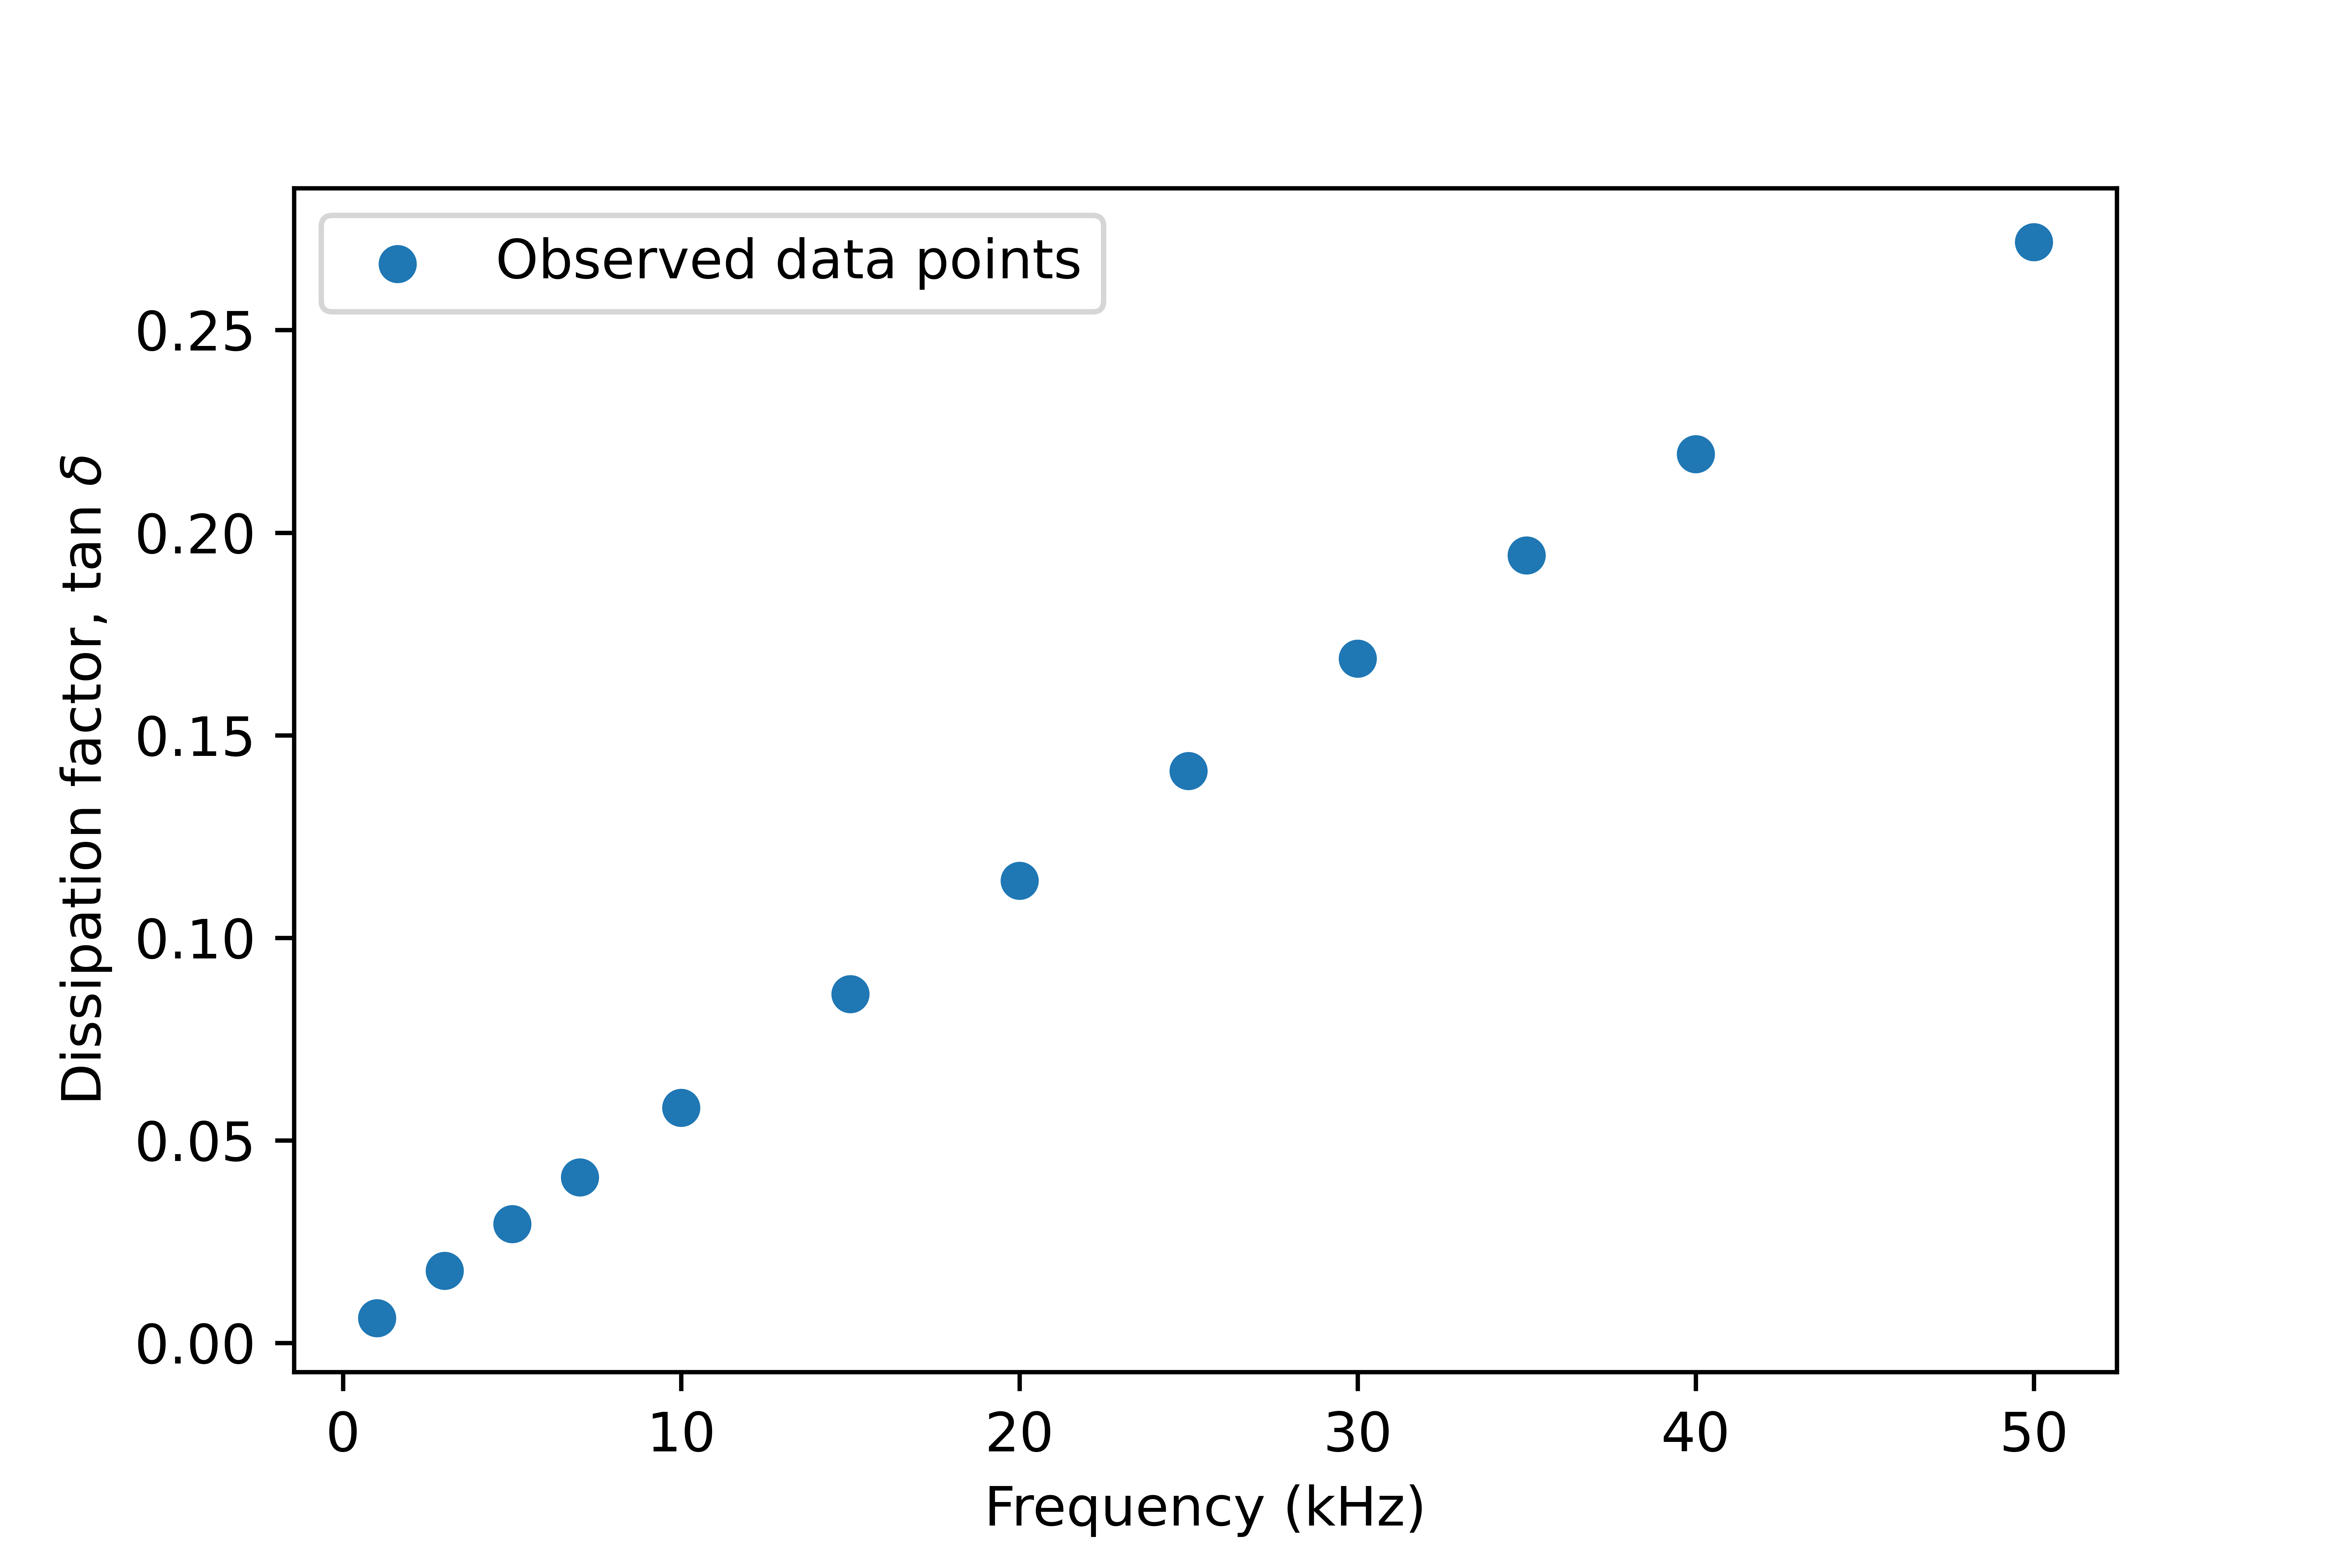
\includegraphics[scale = 0.56]{Figures/plot-dissfac.png}
        \caption{Variation of the dissipation factor of barium titanate sample with frequency}
        \label{fig:diss}
    \end{figure}
    




    \begin{table*}[]
    \caption{Variation of dielectric constant of \ce{BaTiO3} with temperature at various frequencies}
    \label{tab:temp-batio3}
    \setlength{\tabcolsep}{4pt}
    \begin{tabular}{@{}ccccccccccccccccc@{}}
    \toprule
    \multirow{3}{*}{\begin{tabular}[c]{@{}c@{}}\textbf{Temperature}\\ ($\si{\celsius}$)\end{tabular}} &  & \multicolumn{15}{c}{\textbf{Operating frequency}} \\ \cmidrule(l){2-17} 
     &  & \multicolumn{3}{c}{$\SI{5}{\kilo \hertz}$} &  & \multicolumn{3}{c}{$\SI{15}{\kilo \hertz}$} &  & \multicolumn{3}{c}{$\SI{25}{\kilo \hertz}$} &  & \multicolumn{3}{c}{$\SI{35}{\kilo \hertz}$} \\ \cmidrule(lr){3-5} \cmidrule(lr){7-9} \cmidrule(lr){11-13} \cmidrule(l){15-17} 
     &  & \begin{tabular}[c]{@{}c@{}}$R_4$\\ (\si{\ohm})\end{tabular} & \begin{tabular}[c]{@{}c@{}}$C_1$\\ ($\si{\pico \farad}$)\end{tabular} & \begin{tabular}[c]{@{}c@{}}$\epsilon$\\ ($\si{\pico \farad \per \milli \metre}$)\end{tabular} &  & \begin{tabular}[c]{@{}c@{}}$R_4$\\ (\si{\ohm})\end{tabular} & \begin{tabular}[c]{@{}c@{}}$C_1$\\ ($\si{\pico \farad}$)\end{tabular} & \begin{tabular}[c]{@{}c@{}}$\epsilon$\\ ($\si{\pico \farad \per \milli \metre}$)\end{tabular} &  & \begin{tabular}[c]{@{}c@{}}$R_4$\\ (\si{\ohm})\end{tabular} & \begin{tabular}[c]{@{}c@{}}$C_1$\\ ($\si{\pico \farad}$)\end{tabular} & \begin{tabular}[c]{@{}c@{}}$\epsilon$\\ ($\si{\pico \farad \per \milli \metre}$)\end{tabular} &  & \begin{tabular}[c]{@{}c@{}}$R_4$\\ (\si{\ohm})\end{tabular} & \begin{tabular}[c]{@{}c@{}}$C_1$\\ ($\si{\pico \farad}$)\end{tabular} & \begin{tabular}[c]{@{}c@{}}$\epsilon$\\ ($\si{\pico \farad \per \milli \metre}$)\end{tabular} \\ \cmidrule(r){1-17} 
    50 &  & 1856 & 618.7 & 1758.7 &  & 1798 & 599.3 & 1703.7 &  & 1800 & 600.0 & 1705.6 &  & 1792 & 597.3 & 1698.1 \\
    60 &  & 1858 & 619.3 & 1760.6 &  & 1818 & 606.0 & 1722.7 &  & 1788 & 596.0 & 1694.3 &  & 1750 & 583.3 & 1658.3 \\
    70 &  & 1880 & 626.7 & 1781.4 &  & 1884 & 628.0 & 1785.2 &  & 1816 & 605.3 & 1720.8 &  & 1778 & 592.7 & 1684.8 \\
    80 &  & 1912 & 637.3 & 1811.8 &  & 1880 & 626.7 & 1781.4 &  & 1828 & 609.3 & 1732.2 &  & 1826 & 608.7 & 1730.3 \\
    90 &  & 1958 & 652.7 & 1855.4 &  & 1940 & 646.7 & 1838.3 &  & 1920 & 640.0 & 1819.3 &  & 1842 & 614.0 & 1745.4 \\
    100 &  & 2010 & 670.0 & 1904.6 &  & 1966 & 655.3 & 1862.9 &  & 1940 & 646.7 & 1838.3 &  & 1940 & 646.7 & 1838.3 \\
    110 &  & 2130 & 710.0 & 2018.3 &  & 2076 & 692.0 & 1967.2 &  & 2028 & 676.0 & 1921.7 &  & 1984 & 661.3 & 1880.0 \\
    120 &  & 2314 & 771.3 & 2192.7 &  & 2230 & 743.3 & 2113.1 &  & 2208 & 736.0 & 2092.3 &  & 2190 & 730.0 & 2075.2 \\
    130 &  & 2588 & 862.7 & 2452.3 &  & 2518 & 839.3 & 2386.0 &  & 2504 & 834.7 & 2372.7 &  & 2440 & 813.3 & 2312.1 \\
    140 &  & 2726 & 908.7 & 2583.1 &  & 2658 & 886.0 & 2518.7 &  & 2590 & 863.3 & 2454.2 &  & 2530 & 843.3 & 2397.4 \\
    150 &  & 2514 & 838.0 & 2382.2 &  & 2430 & 810.0 & 2302.6 &  & 2422 & 807.3 & 2295.0 &  & 2378 & 792.7 & 2253.3 \\
    160 &  & 2264 & 754.7 & 2145.3 &  & 2196 & 732.0 & 2080.9 &  & 2192 & 730.7 & 2077.1 &  & 2174 & 724.7 & 2060.0 \\
    170 &  & 2028 & 676.0 & 1921.7 &  & 1992 & 664.0 & 1887.6 &  & 1992 & 664.0 & 1887.6 &  & 1940 & 646.7 & 1838.3 \\
    180 &  & 1866 & 622.0 & 1768.2 &  & 1840 & 613.3 & 1743.5 &  & 1822 & 607.3 & 1726.5 &  & 1812 & 604.0 & 1717.0 \\ \bottomrule
    \end{tabular}
    \end{table*}
    
    \begin{figure}
        \centering
        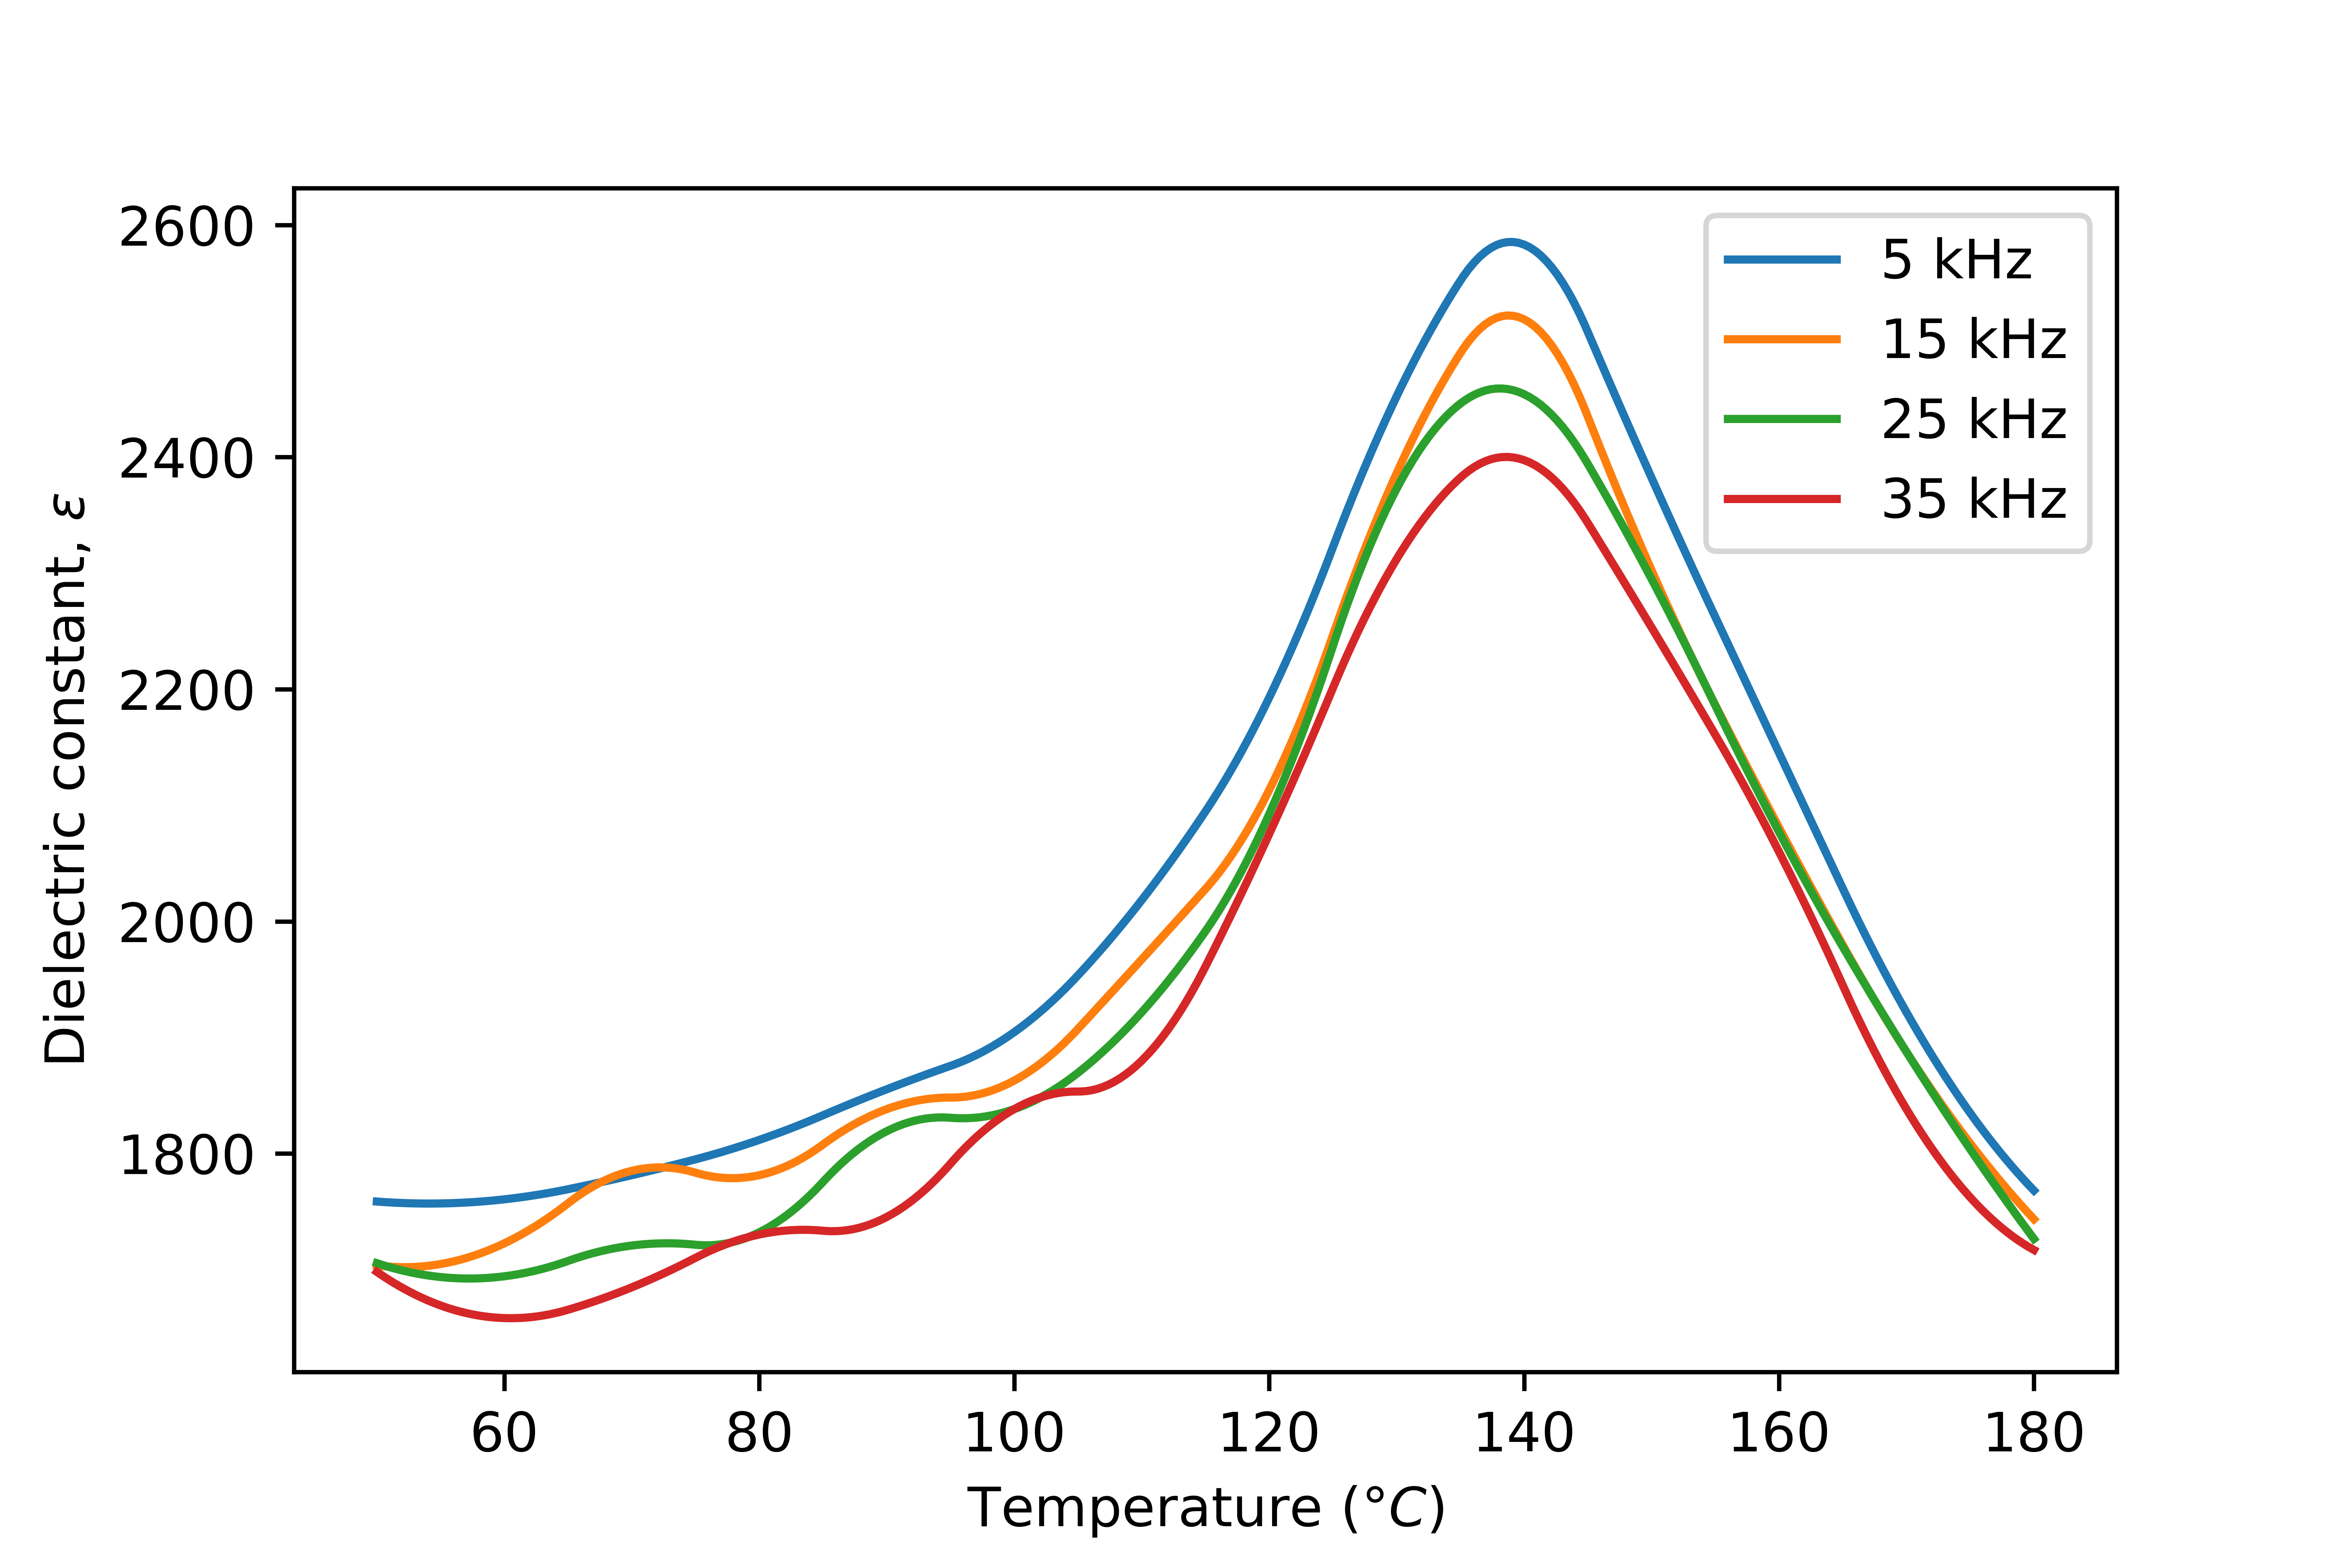
\includegraphics[scale = 0.56]{Figures/plot-curie.png}
        \caption{Variation of dielectric constant of \ce{BaTiO3} with temperature at various frequencies}
        \label{fig:curie}
    \end{figure}


    \begin{table*}[]
    \caption{Log-log plots to study the diffuseness parameter $\delta$ at various frequencies}
    \label{tab:delta}
    \begin{tabular}{@{}ccccccccccccccc@{}}
    \toprule
    \multirow{2}{*}{\begin{tabular}[c]{@{}c@{}}\textbf{Temperature}\\ ($\si{\kelvin}$)\end{tabular}} &  & \multicolumn{2}{c}{\begin{tabular}[c]{@{}c@{}}$\SI{5}{\kilo \hertz}$\\ $\epsilon_{max} = \SI{2583.1}{\pico \farad \per \milli \metre}$\end{tabular}} &  & \multicolumn{2}{c}{\begin{tabular}[c]{@{}c@{}}$\SI{15}{\kilo \hertz}$\\ $\epsilon_{max} = \SI{2518.7}{\pico \farad \per \milli \metre}$\end{tabular}} &  & \multicolumn{2}{c}{\begin{tabular}[c]{@{}c@{}}$\SI{25}{\kilo \hertz}$\\ $\epsilon_{max} = \SI{2454.2}{\pico \farad \per \milli \metre}$\end{tabular}} &  & \multicolumn{2}{c}{\begin{tabular}[c]{@{}c@{}}$\SI{35}{\kilo \hertz}$\\ $\epsilon_{max} = \SI{2397.4}{\pico \farad \per \milli \metre}$\end{tabular}} &  & \multirow{2}{*}{$\ln (T-T_C)$} \\ \cmidrule(lr){3-4} \cmidrule(lr){6-7} \cmidrule(lr){9-10} \cmidrule(lr){12-13}
     &  & \begin{tabular}[c]{@{}c@{}}$\epsilon$\\ \end{tabular} & $\ln (1/\epsilon - 1/\epsilon_{max})$ &  & \begin{tabular}[c]{@{}c@{}}$\epsilon$\\ \end{tabular} & $\ln (1/\epsilon - 1/\epsilon_{max})$ &  & \begin{tabular}[c]{@{}c@{}}$\epsilon$\\ \end{tabular} & $\ln (1/\epsilon - 1/\epsilon_{max})$ &  & \begin{tabular}[c]{@{}c@{}}$\epsilon$\\ \end{tabular} & $\ln (1/\epsilon - 1/\epsilon_{max})$ &  &  \\ \midrule
    423.15 &  & 2382.2 & -10.33 &  & 2302.6 & -10.20 &  & 2295.0 & -10.47 &  & 2253.3 & -10.53 &  & 2.30 \\
    433.15 &  & 2145.3 & -9.45 &  & 2080.9 & -9.39 &  & 2077.1 & -9.51 &  & 2060.0 & -9.59 &  & 3.00 \\
    443.15 &  & 1921.7 & -8.92 &  & 1887.6 & -8.93 &  & 1887.6 & -9.01 &  & 1838.3 & -8.97 &  & 3.40 \\
    453.15 &  & 1768.2 & -8.63 &  & 1743.5 & -8.64 &  & 1726.5 & -8.67 &  & 1717.0 & -8.71 &  & 3.69 \\ \bottomrule
    \end{tabular}
    \end{table*}

    \begin{figure}
        \centering
        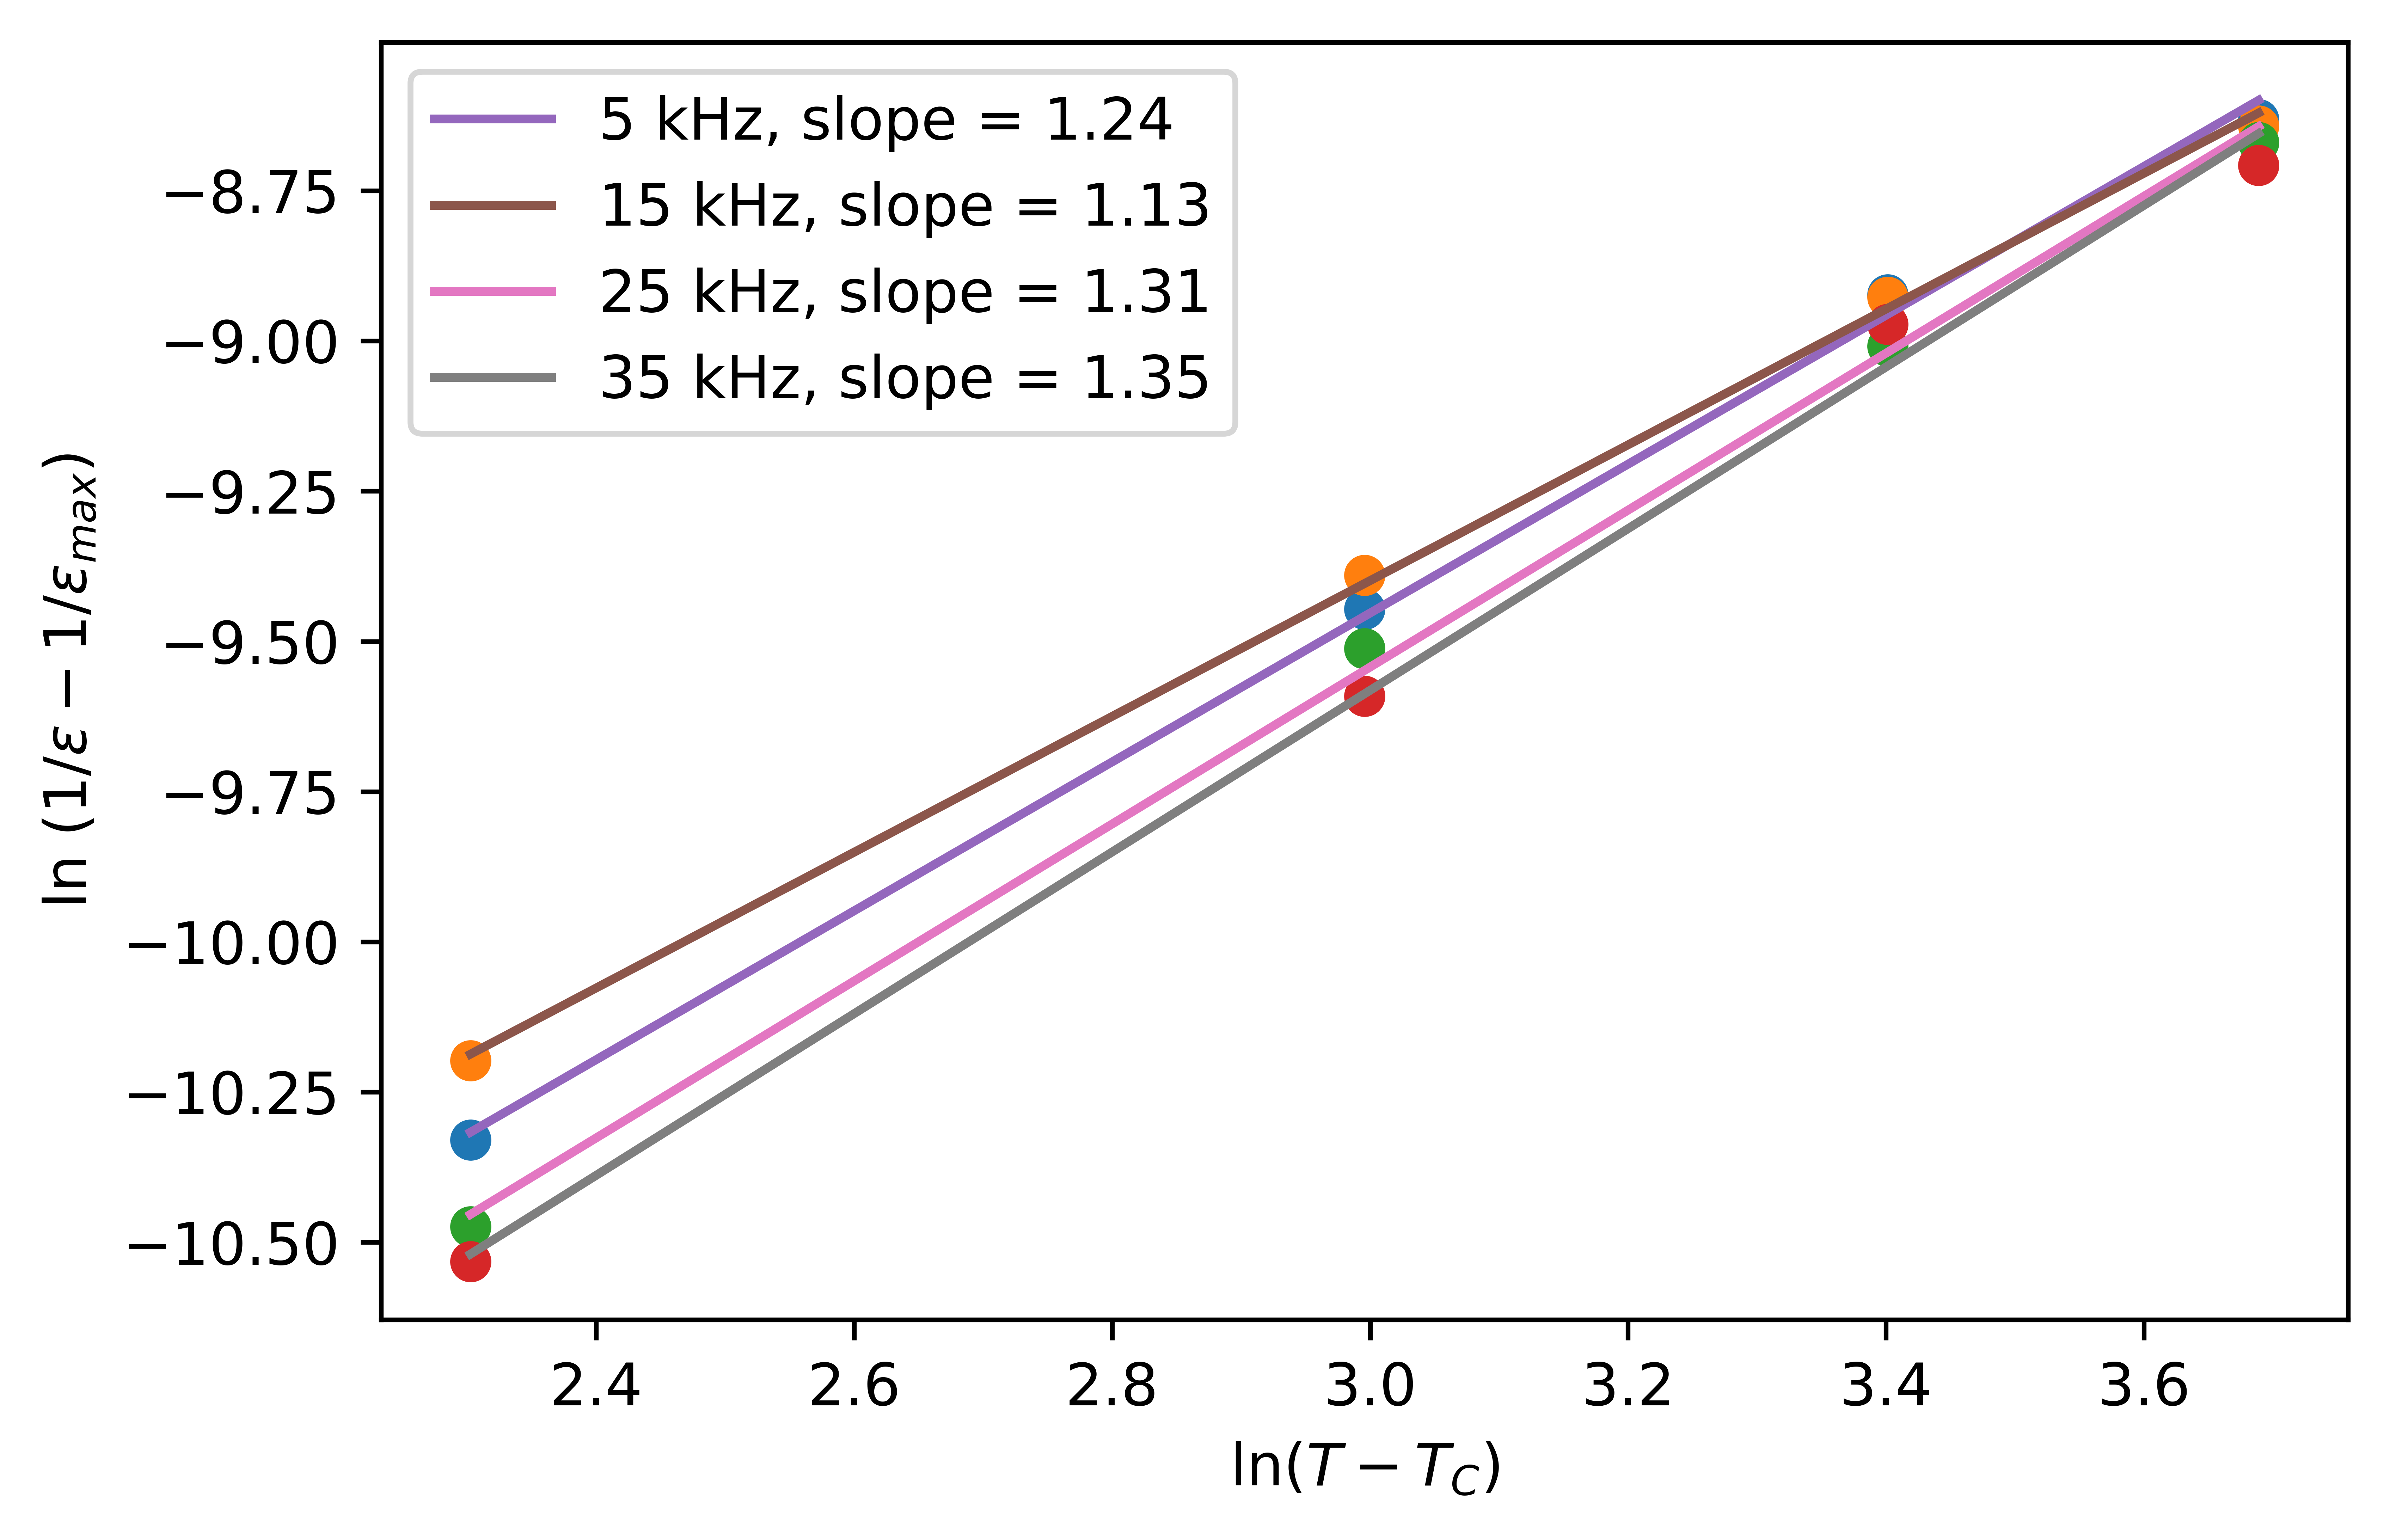
\includegraphics[scale = 0.56]{Figures/plot-diffuse.png}
        \caption{Plot for diffuseness parameter at various frequencies, the slope represents the diffuseness parameter $\delta$}
        \label{fig:delta}
    \end{figure}

\section{Error Analysis}
    Major part of this experiment is concerned with studying the general trend lines, like the effect on the value of dielectric constant when frequency and temperature are changed, that is qualitative analysis. So there is little to no scope in performing rigorous error analysis as we can ascertain the behaviour just by looking the plots and nothing more is required. 
    \par
    Further, figure (\ref{fig:curie}) provides us with value of Curie temperature as around $\SI{140}{\celsius}$. Note that the data entries were erroneously taken in steps of $\SI{10}{\celsius}$ during the range of $\SI{120}{\celsius}$ to $\SI{140}{\celsius}$ instead of steps of $\SI{5}{\celsius}$ as is recommended. This led to the peak appearing much later than expected (around $\SI{140}{\celsius}$, instead of the literature value of $\SI{130}{\celsius}$. It is understood that if the resolution of steps was much higher (less number of steps, more data entries) than the experimental value could have been a lot closer. As the changing of temperature was done using the PID controller oven, it is hard to quantitatively analyse the obtained data set for the error in Curie temperature for such large step values ($\SI{10}{\celsius}$).
    \par
    The log-log plots given in figure (\ref{fig:delta}) do present a opportunity of reasonable quantitative analysis, on the other hand. We are required to find the diffuseness parameter $\delta$ which is, as already calculated, given by the slope of the plots in (\ref{fig:delta}). Error in this slope can be calculated as well. The code for calculating both the slope and its error in given in the Jupyter Notebook at my \href{https://github.com/peakcipher/p345-solid-state-physics-lab}{GitHub}. Upon running the code (which employs the use of popular Python library NumPy), we obtain the diffuseness parameters (with their corresponding uncertainties) as following
    \begin{equation}
    \label{eq:delta}
        \begin{aligned}
            \delta_{5} &= 1.23 \pm 0.03 \\
            \delta_{15} &= 1.13 \pm 0.02 \\
            \delta_{25} &= 1.30 \pm 0.03 \\
            \delta_{35} &= 1.34 \pm 0.06
        \end{aligned}
    \end{equation}
    where $\delta_i$ is the diffuseness parameter for $i$th frequency (in $\si{\kilo \hertz}$).
    
    
    
\section{Results}
\begin{enumerate}
    \item For the multi-layer ceramic capacitor (MLCC), the general trend that was observed was that capacitance (thus dielectric constant) decreases with increase in frequency.
    \item For the disc ceramic capacitor, the general trend that was observed was that capacitance (thus dielectric constant) decreases with increase in frequency.
    \item For \ce{BaTiO3}, the general trend that was observed was that dielectric constant decreases with increase in frequency.
    \item The plot of dissipation factor $\tan \delta$ against frequency was obtained as a straight line. This is not a general trend.
    \item The plots while studying temperature dependence of dielectric constant at various frequencies were obtained as the dielectric constant of \ce{BaTiO3} increased till a critical temperature (the Curie temperature, $T_C$), after which it quickly tapered off.
    \item The experimental Curie temperature was obtained around to be at $\SI{140}{\celsius}$ which is little more than the literature value due to possible reason in taking reading with larger steps than is recommended.
    \item The straight line plots to find diffuseness parameter, $\delta$, were obtained as expected with all $\delta$ values lying between 1 and 2 (as is expected) according to equation (\ref{eq:delta}).
\end{enumerate}

\section{Discussions}
\begin{enumerate}
    \item Dielectric dispersion is the dependence of the permittivity of a dielectric material on the frequency of an applied electric field. Because there is a lag between changes in polarisation and changes in the electric field, the permittivity of the dielectric is a complicated function of frequency of the electric field. Dielectric dispersion is very important for the applications of dielectric materials and for the analysis of polarisation systems.
    \item When the frequency becomes higher dipolar polarisation can no longer follow the oscillations of the electric field in the microwave region, ionic polarisation and molecular distortion polarisation can no longer track the electric field past the infrared or far-infrared region and electronic polarisation loses its response in the ultraviolet region.
    \item Dielectric loss quantifies a dielectric material's inherent dissipation of electromagnetic energy.
    \item The Curie temperature is originally discussed as the temperature above which certain materials lose their permanent magnetic properties, which can (in most cases) be replaced by induced magnetism.
    \item The diffuseness parameters relations are valid in the paraelectric phase, i.e., beyond the Curie temperature.
    \item This aspect which is a structural phase change [Tetragonal to Cubic in the case of BT] with temperature therefore does not depend on the frequency.
    \item The value of the dielectric constant however decreases as the frequency increases in conformity with the results.
    \item The general trend of dielectric constant decreasing with frequency in the case of \ce{BaTiO3} is contributed by space charge polarization caused by mobile charge carriers whose motion is impeded by interface due to a grain or phase boundary.
    \item The general trend of the dissipation factor plot can be explained by the increase with frequency reflects the increase in friction between dipoles due to their inability to follow up the first variation of the applied alternating electric field.
\end{enumerate}

\section{Conclusions}
\begin{enumerate}
    \item In most cases, the results so obtained were satisfactory.
    \item As a precautionary measure, the reading for temperature part must be taken in small steps around the expected value of Curie temperature for better results.
    \item The Schering bridge apparatus often gives the resistance values which are edge on the switch between 1K, 2K or 3k dials. This can lead to some errors as exact value is hard to determine.
    \item The spring loaded probe should be allowed to rest on the sample very gently, otherwise it may damage the conducting surface of the sample or even break the sample.
\end{enumerate}

\nocite{*}
%\bibliography{bibliography}% Produces the bibliography via BibTeX.

\end{document}
%
% ****** End of file aipsamp.tex ******